\documentclass{article}

% Pass options to natbib to use the references.bib file
\PassOptionsToPackage{numbers, compress}{natbib}

% ready for submission
% \usepackage{neurips_2025}

% to compile a preprint version, e.\item \emph{Runtime Scaling}: Repair time scales roughly linearly with set size (10~s $\rightarrow$ 50~s).\item \emph{Runtime Scaling}: Repair time scales roughly linearly with set size (10\,s $\rightarrow$ 50\,s).., for submission to arXiv, add add the
% [preprint] option:
    % \usepackage[preprint]{neurips_2025}

% to compile a camera-ready version, add the [final] option, e.g.:
    \usepackage[final]{neurips_2025}

% to avoid loading the natbib package, add option nonatbib:
%    \usepackage[nonatbib]{neurips_2025}

\usepackage[utf8]{inputenc} % allow utf-8 input
\usepackage[T1]{fontenc}    % use 8-bit T1 fonts
\usepackage{hyperref}       % hyperlinks
\usepackage{url}            % simple URL typesetting
\usepackage{booktabs}       % professional-quality tables
\usepackage{amsmath}        % AMS math symbols and environments
\usepackage{amsfonts}       % blackboard math symbols
\usepackage{nicefrac}       % compact symbols for 1/2, etc.
\usepackage{microtype}      % microtypography
\usepackage{xcolor}         % colors
\usepackage{booktabs} % For better looking tables
\usepackage{longtable} % For tables that might span multiple pages
\usepackage{graphicx}      % for including images

\title{Informed Repair of Deep Neural Networks}

\begin{document}

\author{
	Akshat Adsule \\
	University of California, Davis \\
	\texttt{aadsule@ucdavis.edu}
	\And
	Darroll Saddi \\
	University of California, Davis \\
	\texttt{dwsaddi@ucdavis.edu}
	\And
	Suyash Goel \\
	University of California, Davis \\
	\texttt{sngoel@ucdavis.edu}
}

\maketitle

% \begin{abstract}
%     Work in Progress
% \end{abstract}

\section{Introduction}

Deep neural networks (DNNs) have become increasingly prevalent in modern applications.
DNNs have seen use in virtually every field from air traffic control to self-driving vehicles.
However, these models are not infallible and do produce mistakes, which could prove disastrous given the model's application.

Recent research \cite{nawas_provable_2024, sotoudeh_provable_2021, tao_architecture-preserving_2023} has explored methods of repairing DNNs once incorrect inputs are identified.
Repair techniques have the goal of correcting the model's behavior on a specified set of inputs, often referred to as the repair set.
The goal of many existing techniques is to adjust network weights and biases while satisfying the conditions of: (i) provable, (ii) generalizing, (iii) architecture-preserving, (iv) scalable, and (v) local repair.
In other words, these techniques typically aim to minimally adjust the network's parameters to correct its behavior on the specified repair set, often while providing formal guarantees on the outcome for those inputs or related input regions.
While methods that satisfy some or even all of these conditions exist, most require user intervention to select the repair set and which layers of the network should be affected.
Thus, in practice, applying these repair methods reveals significant ambiguities that can affect the quality and efficiency of the repair.

Take, for example, APRNN, the method proposed in \cite{tao_architecture-preserving_2023} that offers provable, architecture-preserving repair over specified input regions (V-polytopes).
APRNN achieves all the previously stated conditions (i-v), and works by provably repairing the network's weights and biases up to a chosen layer.
This involves modifying network weights starting primarily at that chosen layer and adjusting biases in subsequent layers.

While effective, APRNN includes critical ambiguities in practice, mainly as a result of the user needing to select the starting layer or affected layers for weight and bias adjustment.
The paper itself doesn't prescribe how to choose affected layer, and this choice can significantly impact the repair's effectiveness, efficiency, and efficacy.
The choice of repair set, which defines the repair polytope, is also left to the user -- fundamentally determining the target behavior of the repair.
The composition and scope of this set influence the repair outcome and how well the fix generalizes to similar, unseen inputs.
This situation is not ideal because these choices can be arbitrary and greatly impact the quality of the repair.

This paper aims to investigate and develop heuristics to guide the DNN repair process, specifically addressing the ambiguities highlighted above in methods like APRNN.
By providing data-driven or structurally-informed ways to make these choices, we seek to enable more efficient and informed repairs of DNNs.
We propose to explore and evaluate various heuristics, including but not limited to:

\newpage

% \subsubsection*{Layer Selection Heuristics}
\underline{Layer Selection Heuristics:}
\begin{description}
	\item[Activation-Based] Selecting the start layer based on metrics calculated across the repair set, such as the layer exhibiting the highest average activation magnitude or the highest variance in activations.
	\item[Gradient/Sensitivity-Based] Identifying layers where parameters show the most sensitivity (e.g., largest gradient norms) with respect to the inputs in the repair set, indicating layers most influential on the incorrect output.
	\item[Change-Based (for Adversarial Inputs)] Selecting the layer whose activations or feature representations changed most drastically between the original and adversarial inputs in the repair set.
	\item[Feature-Similarity Based] Choosing a layer where the internal representations of the inputs within the repair set are most similar, suggesting a point of unified processing relevant to the required fix.
	\item[Layer Type/Position] Simple heuristics such as always choosing the first fully-connected layer after convolutional blocks, or the penultimate layer.
	\item[Brute Force] Exhaustively evaluating all layers and selecting the one that yields the best repair outcome, though this is computationally expensive.
\end{description}

\underline{Repair Set Analysis}
\begin{description}
	\item[Diversity] Evaluating the diversity of the repair set, such as the number of unique classes or the distribution of inputs across the input space.
	\item[Concentration] Analyzing the concentration of points defining the polytope, such as the number of points needed to define a convex hull or the dimensionality of the convex hull.
	\item[Size] Considering the size of the repair set, including the number of points and the dimensionality of the input space.
\end{description}

% We plan to also evaluate these heuristics on the architecture of [] trained on the [] dataset.
% We also hope to use the following metrics to evaluate the heuristics:

% \underline{Evaluation Metrics:}
% \begin{description}
%     \item[Repair Success Rate] The percentage of inputs in the repair set for which the model produces the correct output after repair.
%     \item[Generalization] The model's performance on unseen inputs similar to those in the repair set, measured by accuracy or other relevant metrics.
%     \item[Locality] The extent to which the repair minimally affects the model's behavior on inputs outside the repair set, often quantified by changes in the model's predictions or parameter values.
%     \item[Efficiency] The computational cost of the repair process, including time and resources required.
%     \item[Scalability] The ability of the repair method to handle larger models or repair sets without significant degradation in performance or efficiency. [May not be able to measure this in this project]
% \end{description}

This project enhances AI trustworthiness by making the crucial process of model repair, itself a method for increasing trust after failures—more efficient and informed.
Current repair techniques can involve arbitrary choices, leading to unpredictable outcomes.
By developing heuristics to guide decisions within the repair process, such as selecting the optimal network layer for modification, we enable more systematic, reliable, and effective correction of identified flaws.
This ultimately increases confidence in the robustness and safety of AI systems by ensuring that necessary fixes are applied more predictably and with a better understanding of their potential impact.

\section{Experimental Setup}

The experiments are designed to answer the primary research question:
\textit{How do different heuristics for layer selection (e.g., activation-based, gradient-based) and repair set analysis (e.g., diversity, concentration) influence the effectiveness, generalization, locality, and efficiency of DNN repair techniques like APRNN?}
We aim to determine which heuristics provide the most significant improvements over arbitrary or naive selection strategies.

\subsection{Models \& Datasets}

\subsubsection{Selected Architectures}
We aim to identify heuristics for a wide variety of model types and repair types.
We choose models that are frequenty used in most machine learning tasks.
These include:

\begin{description}
	\item[Multi-Level Perceptrons (MLPs)] {
		MLPs are foundational neural networks with hidden layers, fully connected neurons, and non-linear activations used widely for classification and regression tasks.
		}
	\item[Convolutional Neural Networks (CNNs)] {
		CNNs excel at processing grid-like data, especially images, by using convolutional layers to learn spatial feature hierarchies.
		CNNs are most used for vision tasks such as classification, object detection, and segmentation.
		}
\end{description}

\subsubsection{Selected Models}

For experimentation purposes, we choose the following pre-trained models for each aforementioned model architecture.
We picked models that are relativly well-established for their respective tasks.
We also purposefully choose smaller models for ease of experimentation.
However, we still expect our results to apply to larger and more complex models.

Our chosen models are:
\begin{description}
	\item[Clustering MLP] {
		To simulate a classic use of MLPs, we implemented a simple supervised clustering problem, we can create a simple MLP model that is trained to classify points in a 2D space into two clusters.
		}
	\item[AlexNet \cite{alexnet}] AlexNet is a CNN architecture that achieved remarkable success in the ImageNet competition by using deep learning techniques, including ReLU activations and dropout for regularization.
\end{description}

\subsubsection{Selected Datasets}
We will use the following datasets for our experimentation that correspond to the selected pre-trained models.

\begin{description}
	\item[Custom Clusering Dataset] {
		We will use the \texttt{make\_moons} function from \texttt{sklearn.datasets} to generate a dataset, where an MLP will be insufficiently trained on this dataset to classify the points into two clusters.
		By either increasing the complexity of the dataset (e.g. the number of points, noise), or by not training the MLP enough, we can apply our heuristics to see if any significant improvements can be made, or if there are any significant differences between the heuristics.
		By training an MLP on a supervised (known labels) clustering task, we can create a simple MLP model that is trained to classify points in a 2D space into two clusters.
		}
	\item[CIFAR-10 \cite{cifar_10}] {
		CIFAR-10 is a widely used image dataset consisting of 60,000 32x32 color images in 10 classes, with 6,000 images per class.
		CIFAR-10 is used by both AlexNet.
		}
\end{description}

\subsubsection{Summary}

The following table summarizes the models and datasets we use in our experimentation.

\begin{longtable}{p{0.25\textwidth} p{0.3\textwidth} p{0.35\textwidth}}
	\toprule
	\textbf{Architecture} & \textbf{Model}          & \textbf{Dataset}          \\
	\midrule
	\endhead
	\bottomrule
	\endfoot
	\bottomrule
	\endlastfoot
	MLPs                  & Custom Clustering Model & Custom Clustering Dataset \\
	\midrule
	CNNs                  & AlexNet \cite{alexnet}  & CIFAR-10 \cite{cifar_10}  \\
\end{longtable}

\subsection{Evaluation Metrics}
We will evaluate the heuristics based on the following metrics:
\begin{description}
	\item[Repair Success Rate] The percentage of inputs in the repair set for which the model produces the correct output after repair.
	\item[Generalization] The model's performance on unseen inputs similar to those in the repair set, measured by accuracy or other relevant metrics.
	\item[Locality] The extent to which the repair minimally affects the model's behavior on inputs outside the repair set, often quantified by changes in the model's predictions or parameter values.
	\item[Efficiency] The computational cost of the repair process, including time and resources required.
	\item[Scalability] The ability of the repair method to handle larger models or repair sets without significant degradation in performance or efficiency.
\end{description}

\section{Results and Discussion}

\subsection{Layer Selection Heuristics}

\subsection{Repair Set Analysis}
We conducted two complementary suites of experiments to understand the trade-offs inherent in repairing AlexNet on CIFAR-10:

\begin{description}
	\item[Deterministic ("full-set") repair]in which we solve a single repair problem over an entire edit set of varying size and homogeneity.
	\item[Stochastic ("incremental") repair]in which we perform repeated, small-batch repair passes—carrying forward the model between passes—so as to trade batch size, number of passes, and homogeneity against overall fidelity.
\end{description}

We measured how each strategy trades off global test accuracy against local repair accuracy, how repair‐set size and batch size affect performance, and how repeated fixes accumulate.

We conducted comprehensive experiments on AlexNet trained on CIFAR-10 to evaluate different repair strategies and understand the fundamental trade-offs between local correctness and global performance preservation. Our experiments used a pretrained AlexNet model with baseline test accuracy of 72.08\% on CIFAR-10.

\subsubsection{Repair Set Size Impact}

Our experiments demonstrate that larger repair sets consistently lead to worse performance across all metrics. As repair set size increases from 10 to 200 examples, we observe dramatic degradation in success rates, increased accuracy drawdown, and longer repair times.

\begin{figure}[h]
	\centering
	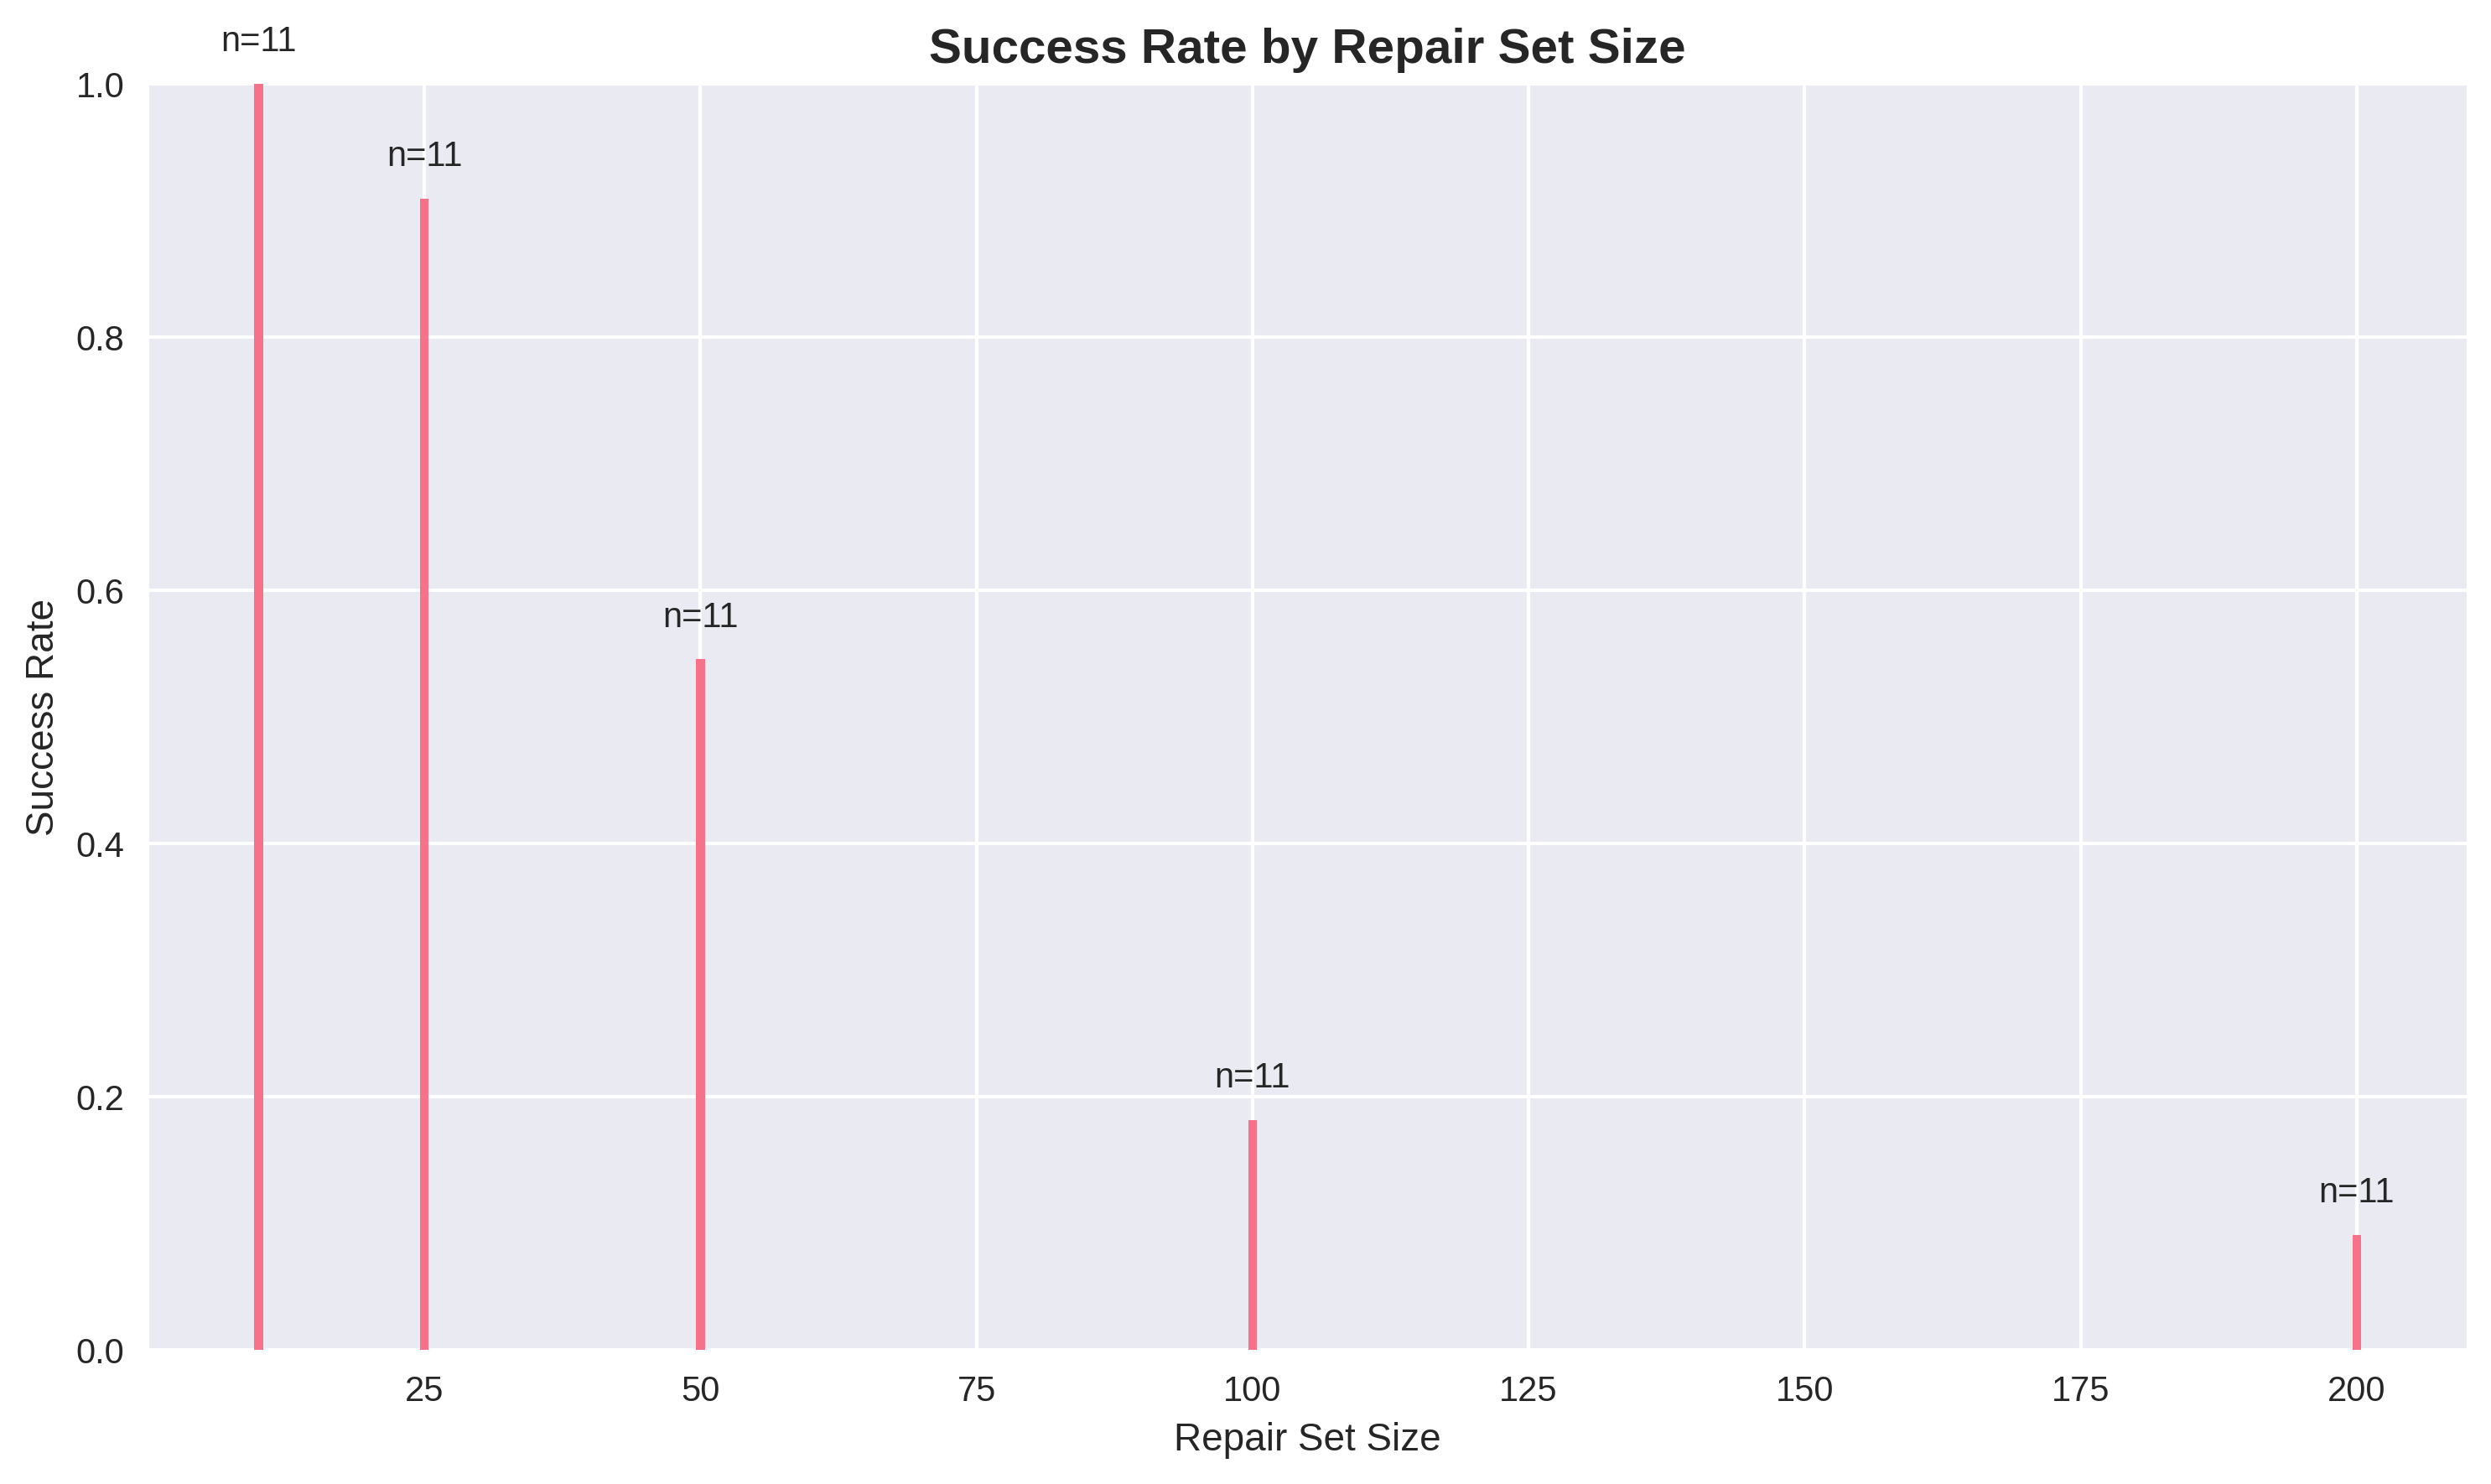
\includegraphics[width=0.8\textwidth]{results/one_shot_analysis/success_rates/success_rate_by_size.png}
	\caption{Success rate by repair set size, showing dramatic degradation in repair feasibility as set size increases beyond 25 examples.}
	\label{fig:success_rate_by_size}
\end{figure}

\begin{figure}[h]
	\centering
	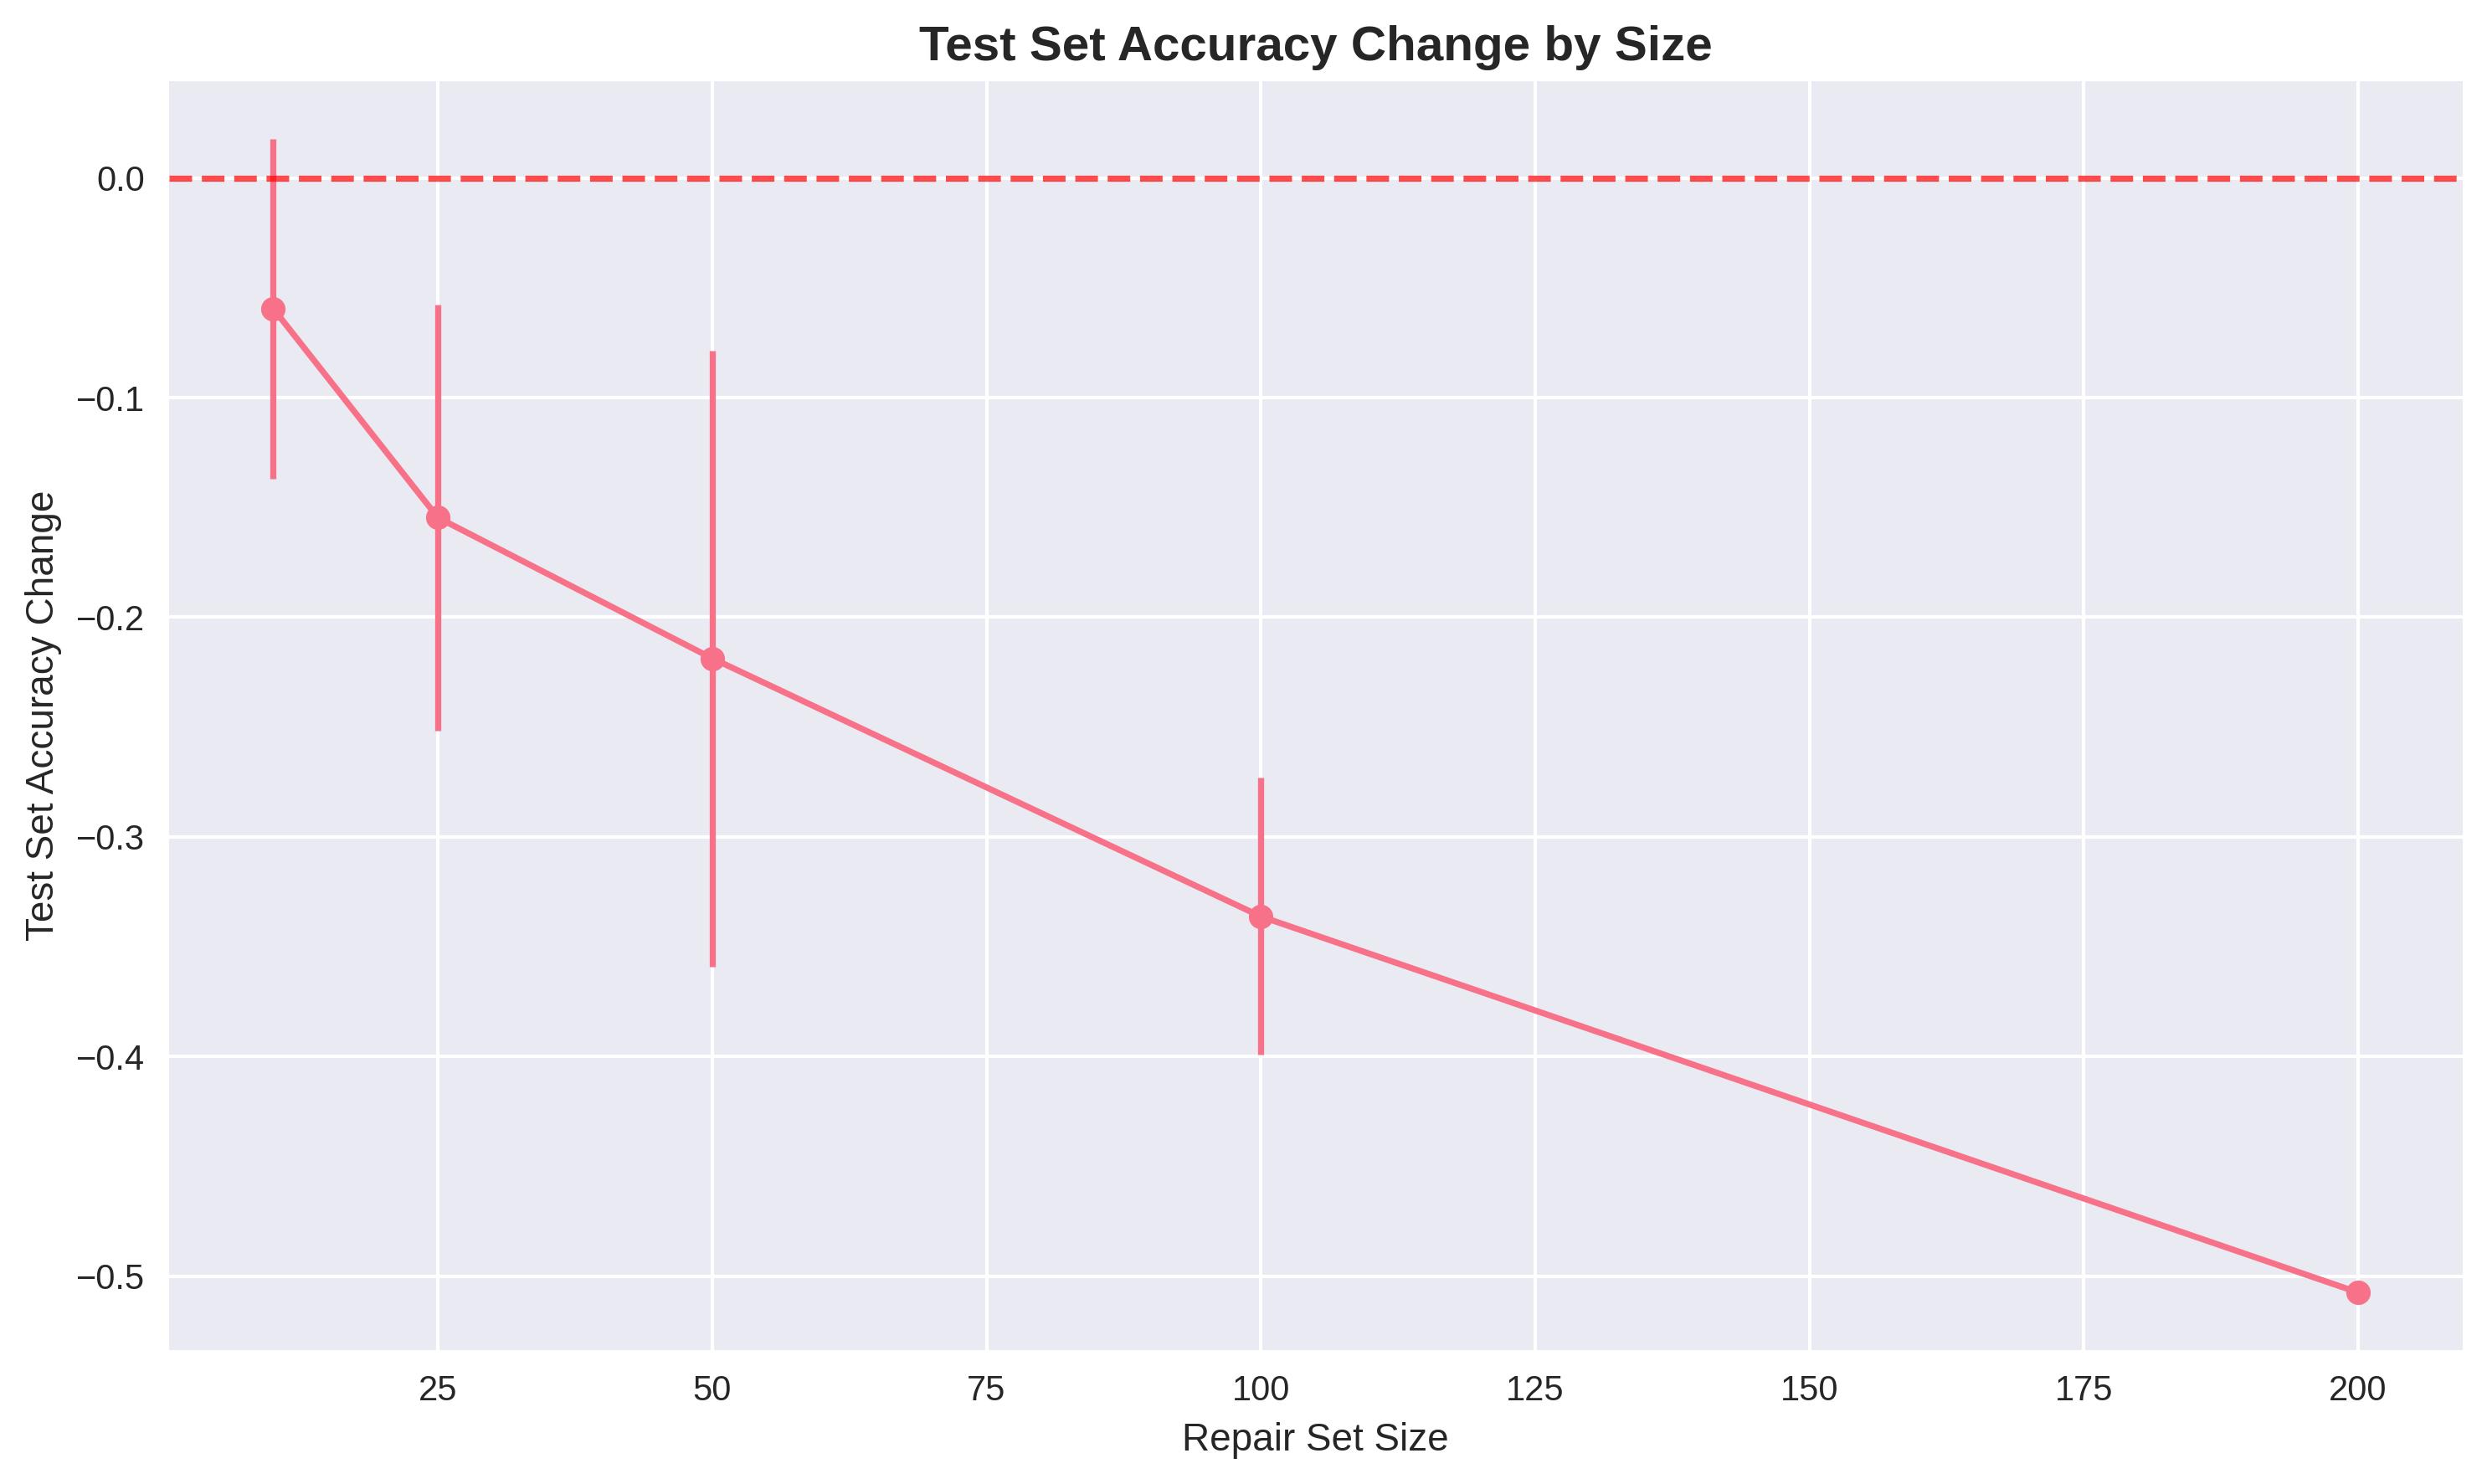
\includegraphics[width=0.8\textwidth]{results/one_shot_analysis/accuracy/accuracy_change_by_size.png}
	\caption{Test set accuracy drawdown by repair set size, demonstrating the severe trade-off between local repair success and global model performance as repair set size increases.}
	\label{fig:accuracy_drawdown_by_size}
\end{figure}

The data shows clear trends across all metrics:
\begin{itemize}
	\item \textbf{Success Rate:} Drops from 100\% for size 10 to just 9.1\% for size 200
	\item \textbf{Accuracy Drawdown:} Increases from minimal impact (~-2.7\%) for small sets to severe degradation (-50.8\%) for large sets
	\item \textbf{Repair Time:} Scales linearly from ~10 seconds to ~50 seconds as set size increases
\end{itemize}

\subsubsection{Repair Set Homogeneity Effects}

Repair set composition significantly impacts both success rates and performance degradation patterns. Class-homogeneous sets consistently outperform misclassified sets across all metrics.

\begin{figure}[h]
	\centering
	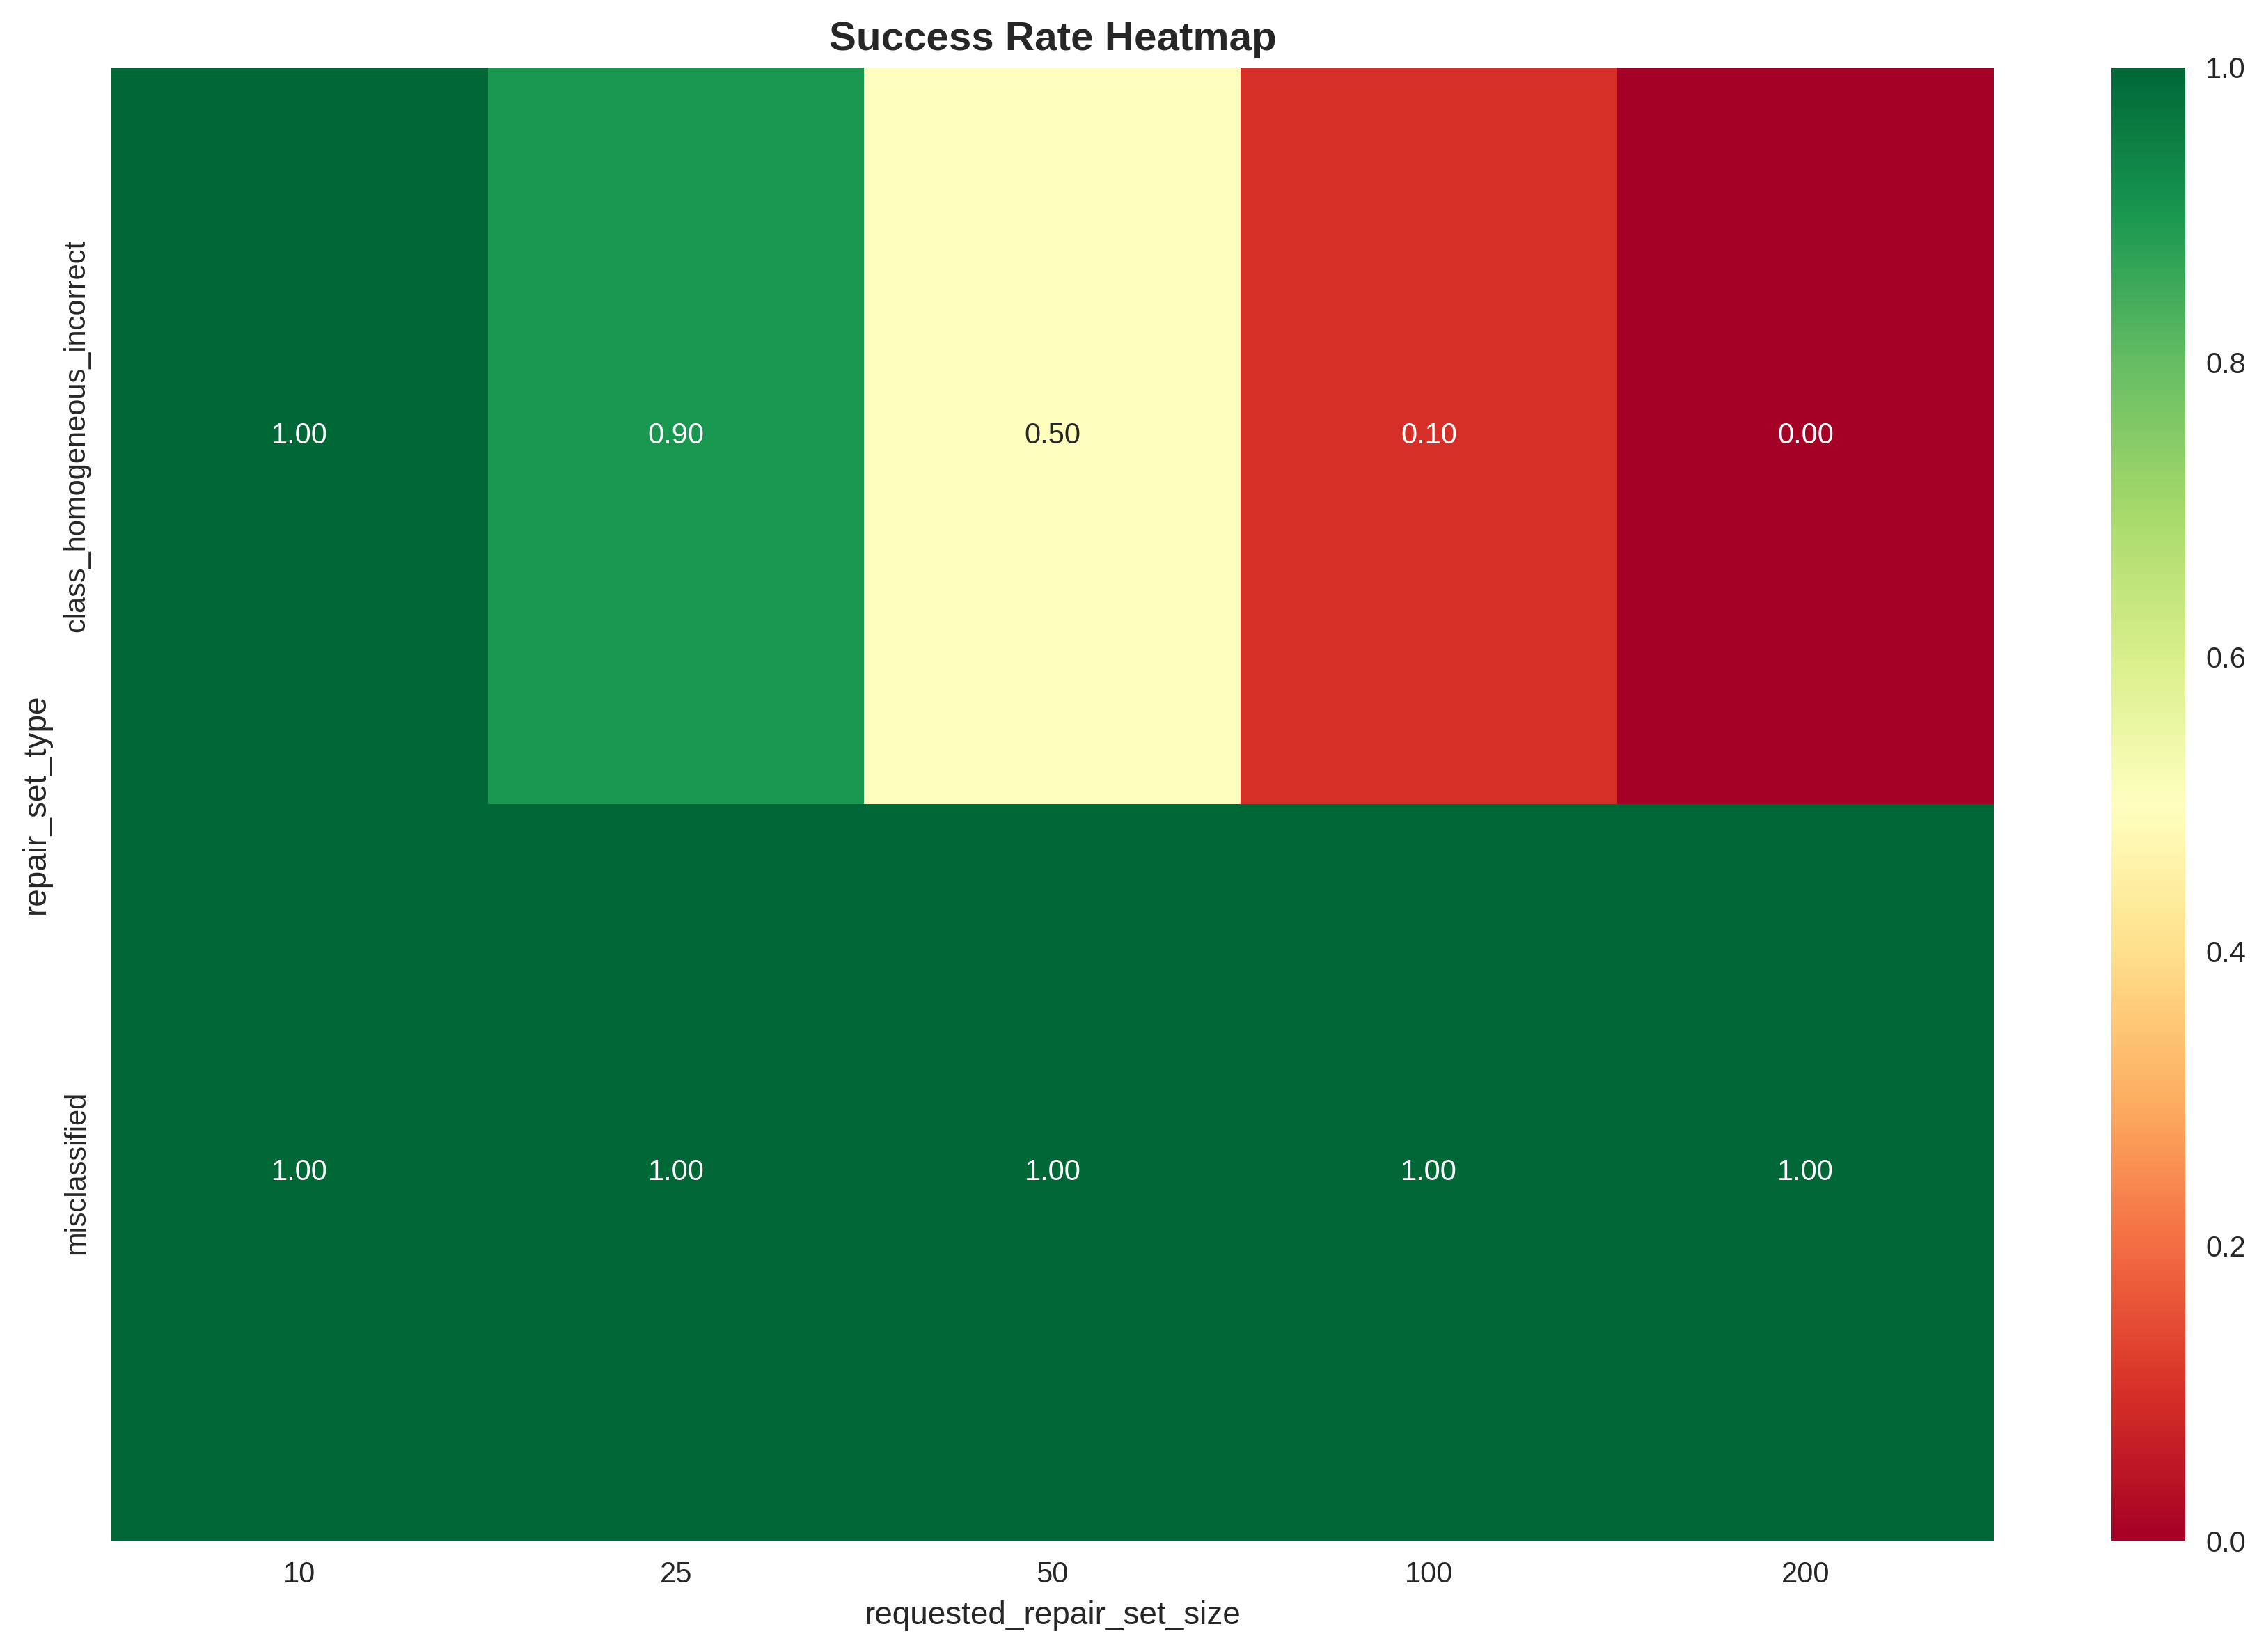
\includegraphics[width=0.8\textwidth]{results/one_shot_analysis/success_rates/success_rate_heatmap.png}
	\caption{Success rate heatmap showing the interaction between repair set type and size, clearly illustrating the feasibility boundaries for different repair strategies.}
	\label{fig:success_rate_heatmap}
\end{figure}

\begin{figure}[h]
	\centering
	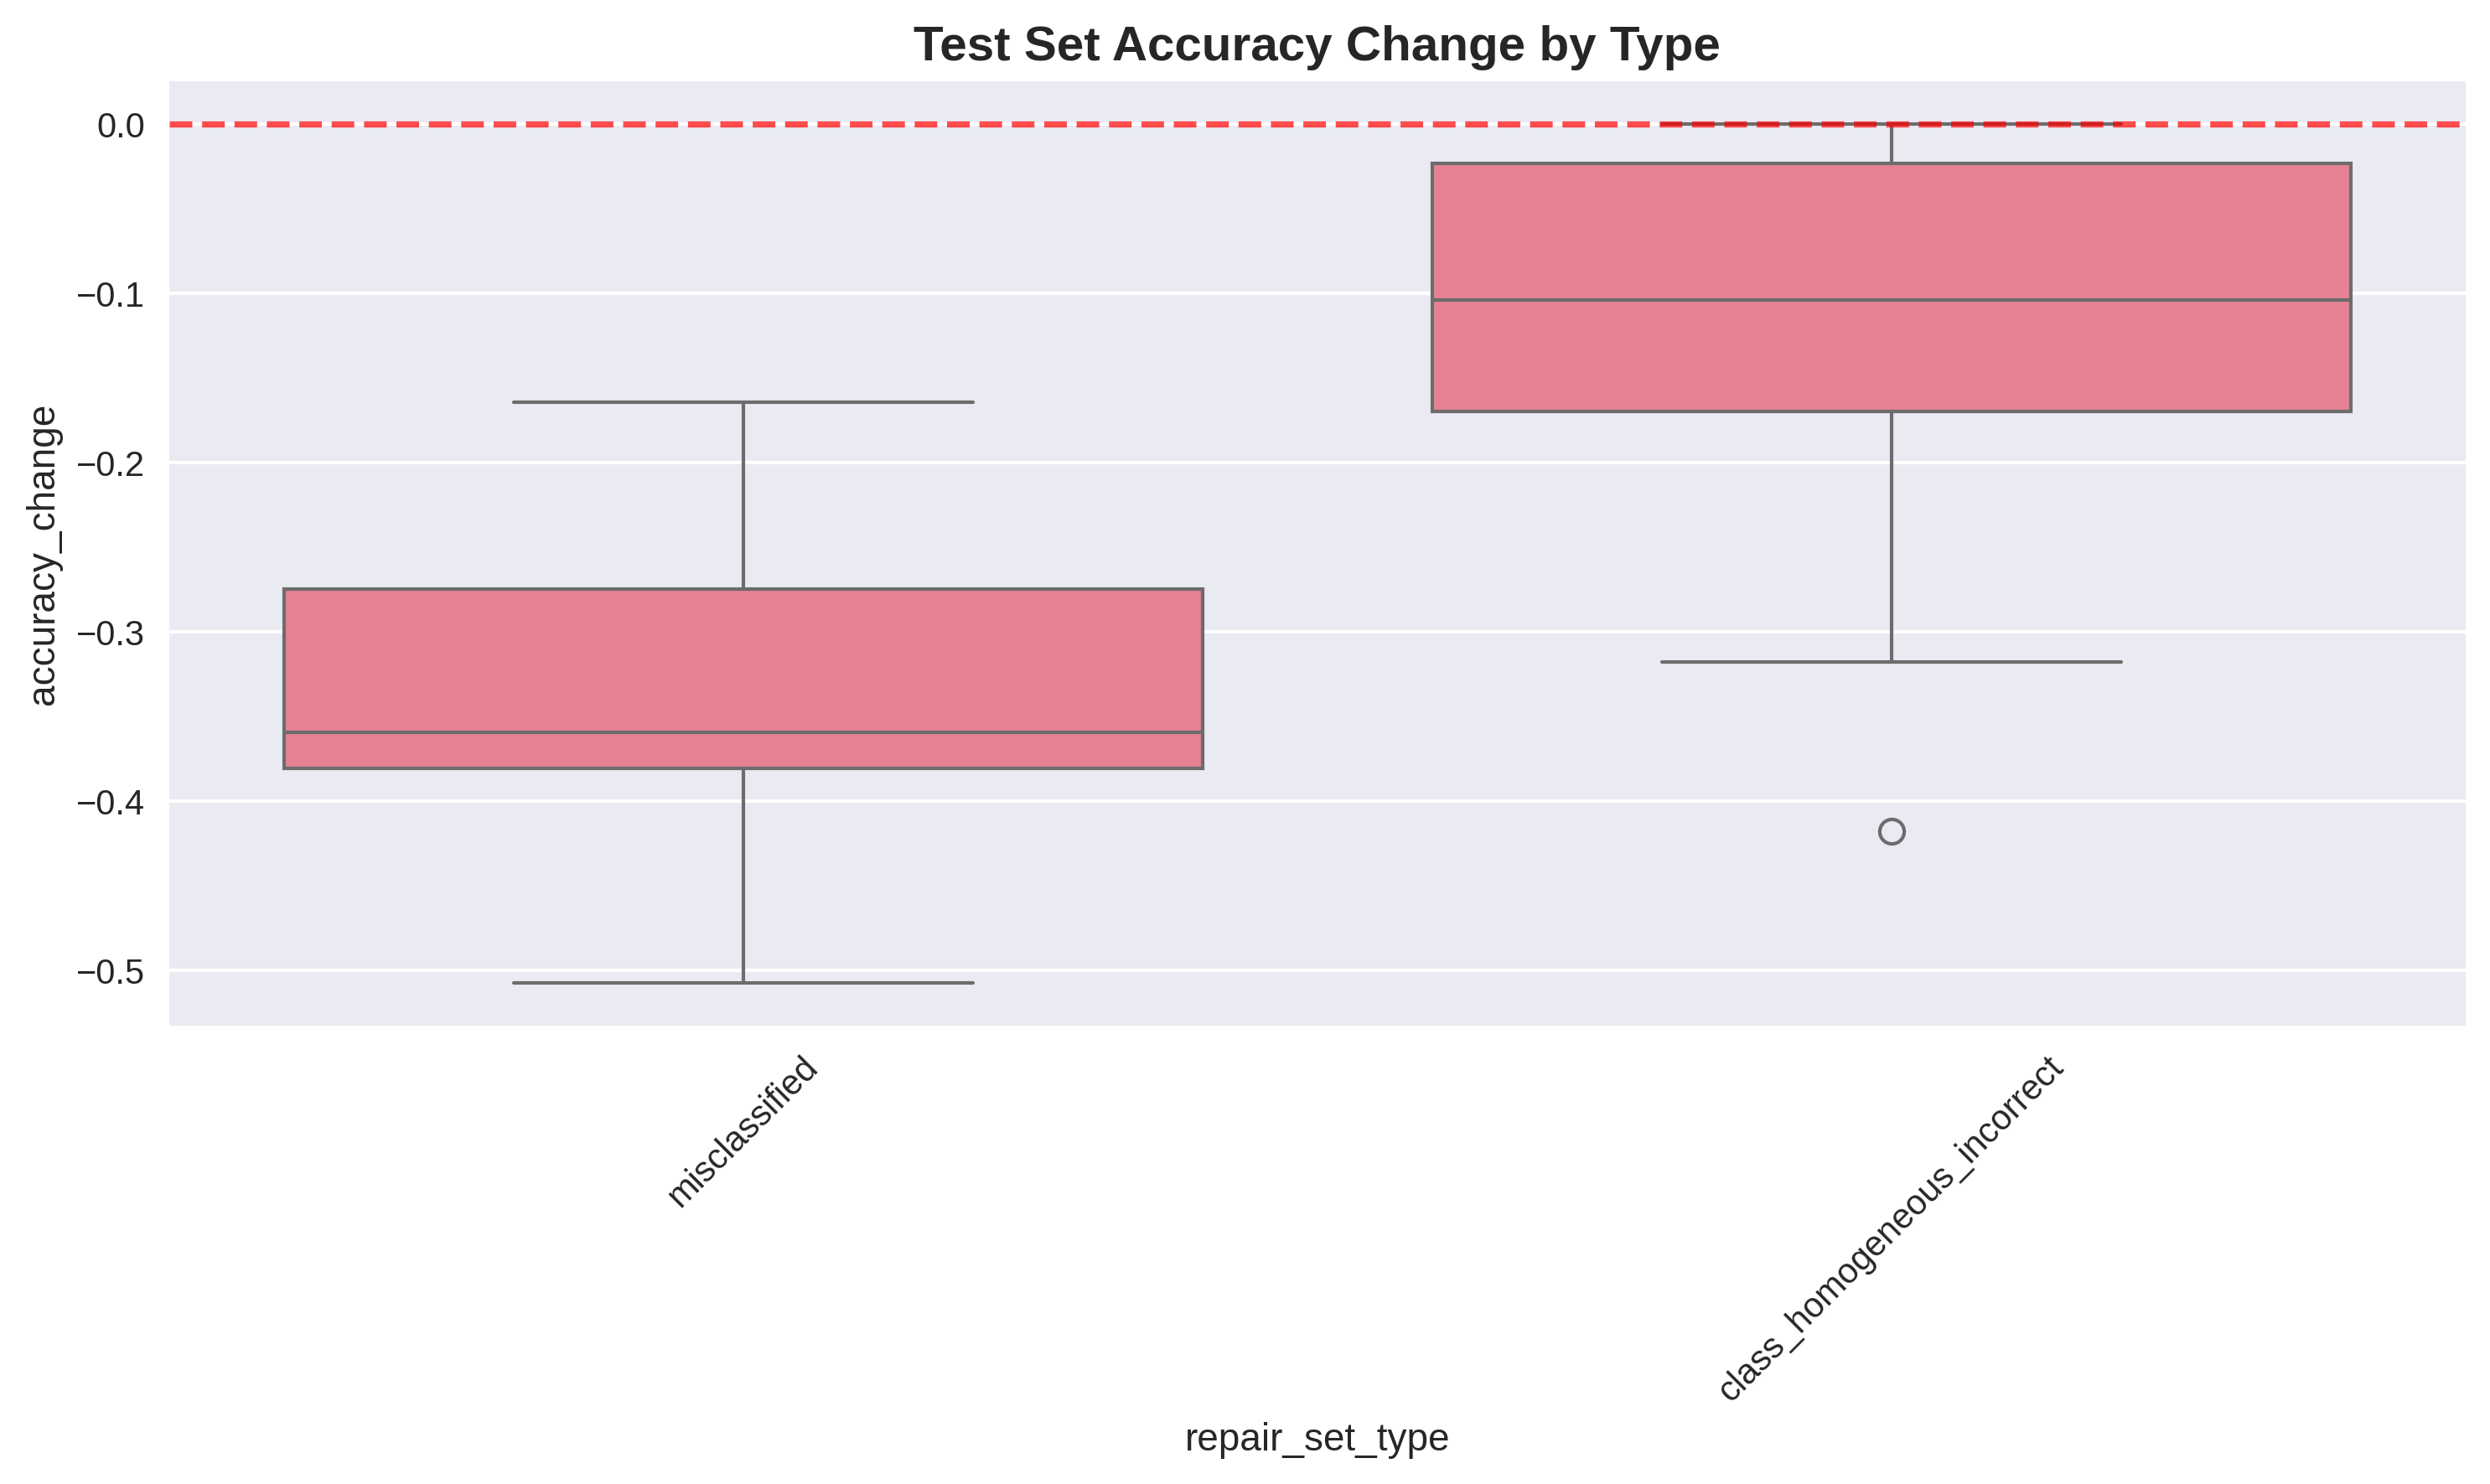
\includegraphics[width=0.8\textwidth]{results/one_shot_analysis/accuracy/accuracy_change_by_type.png}
	\caption{Accuracy drawdown distribution by repair set type, demonstrating that class-homogeneous repairs cause significantly less performance degradation than misclassified repairs.}
	\label{fig:accuracy_change_by_type}
\end{figure}

\subsubsection{Stochastic Repair Efficiency for Class-Homogeneous Sets}

Our stochastic experiments focused on batch sizes of 5 and 10, as batch size 20 resulted in too many infeasible repairs. For class-homogeneous sets, stochastic repair proves highly efficient, achieving rapid convergence to near-perfect repair set accuracy.

\begin{figure}[h]
	\centering
	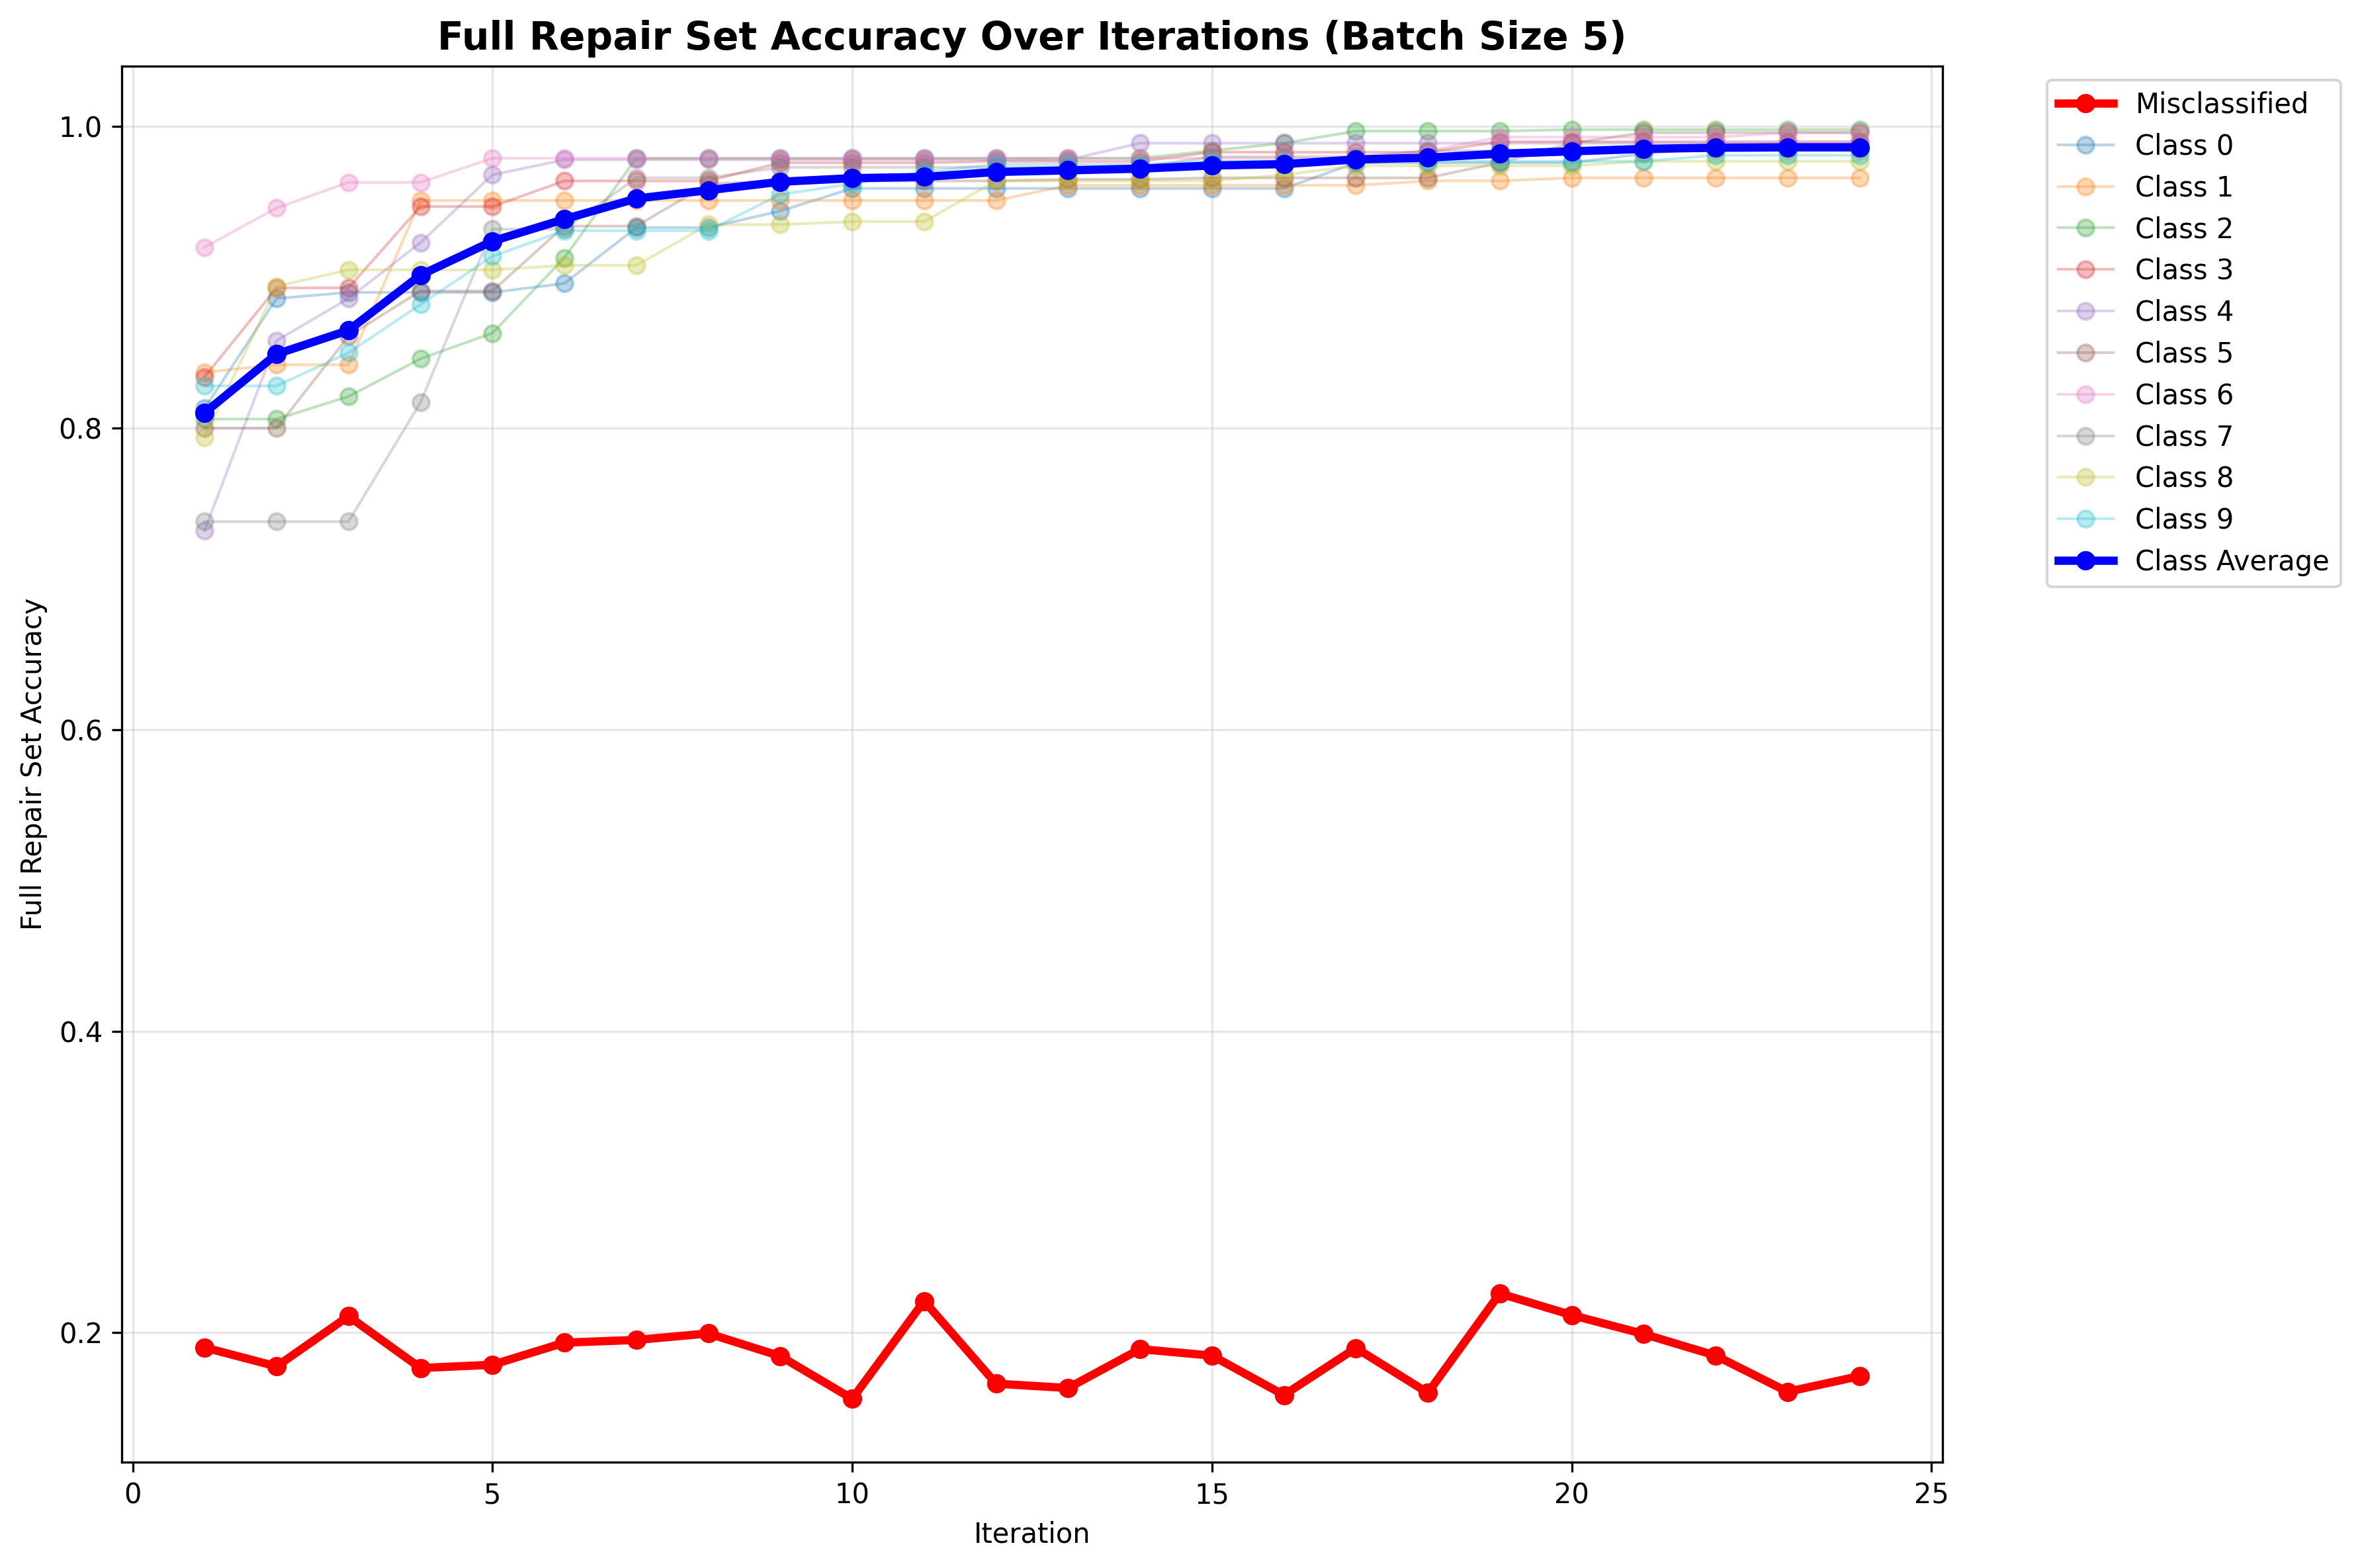
\includegraphics[width=\textwidth]{results/stochastic_analysis/batch_iterations/repair_accuracy_batch_5.png}
	\caption{Repair set accuracy evolution for batch size 5, showing rapid convergence to near-perfect accuracy within 5 iterations for class-homogeneous repairs.}
	\label{fig:repair_convergence_batch_5}
\end{figure}

\begin{figure}[h]
	\centering
	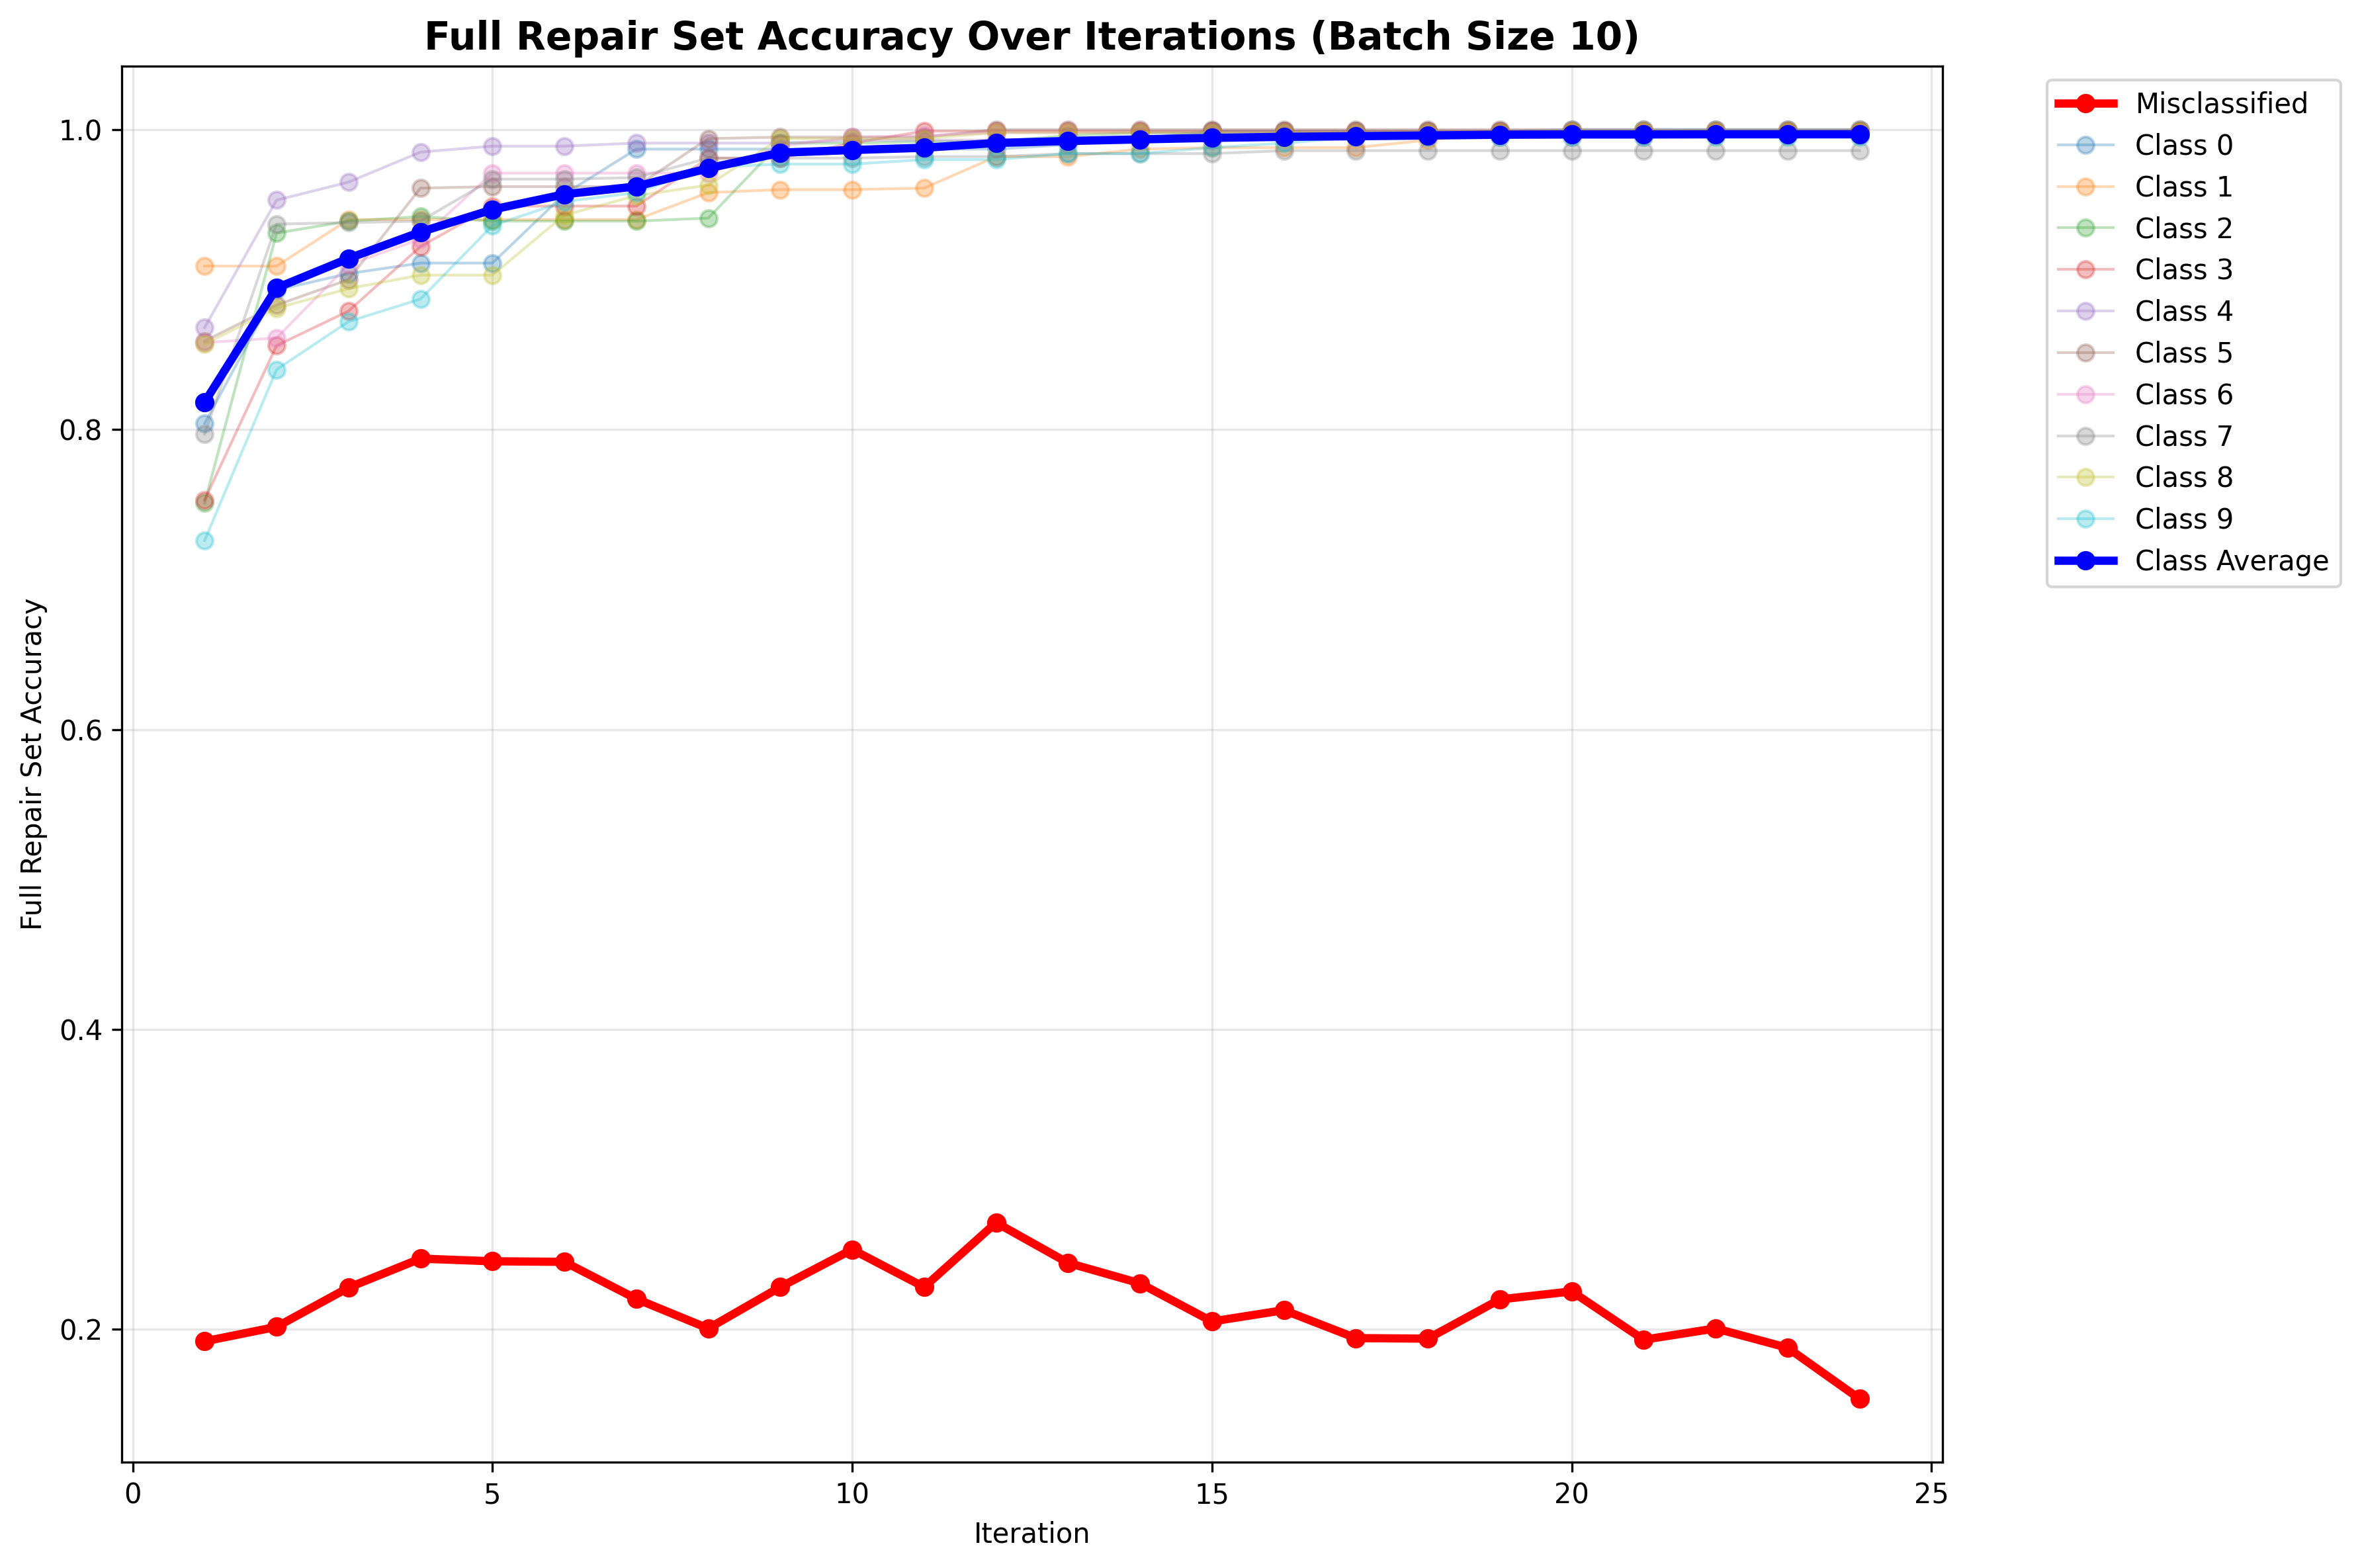
\includegraphics[width=\textwidth]{results/stochastic_analysis/batch_iterations/repair_accuracy_batch_10.png}
	\caption{Repair set accuracy evolution for batch size 10, demonstrating similar rapid convergence patterns to batch size 5.}
	\label{fig:repair_convergence_batch_10}
\end{figure}

\subsubsection{Early Stopping to Reduce Drawdown}

The key insight is that stochastic repair converges to near-perfect repair set accuracy within approximately 5 iterations. Stopping early can significantly reduce global accuracy drawdown while maintaining excellent local repair performance.

\begin{figure}[h]
	\centering
	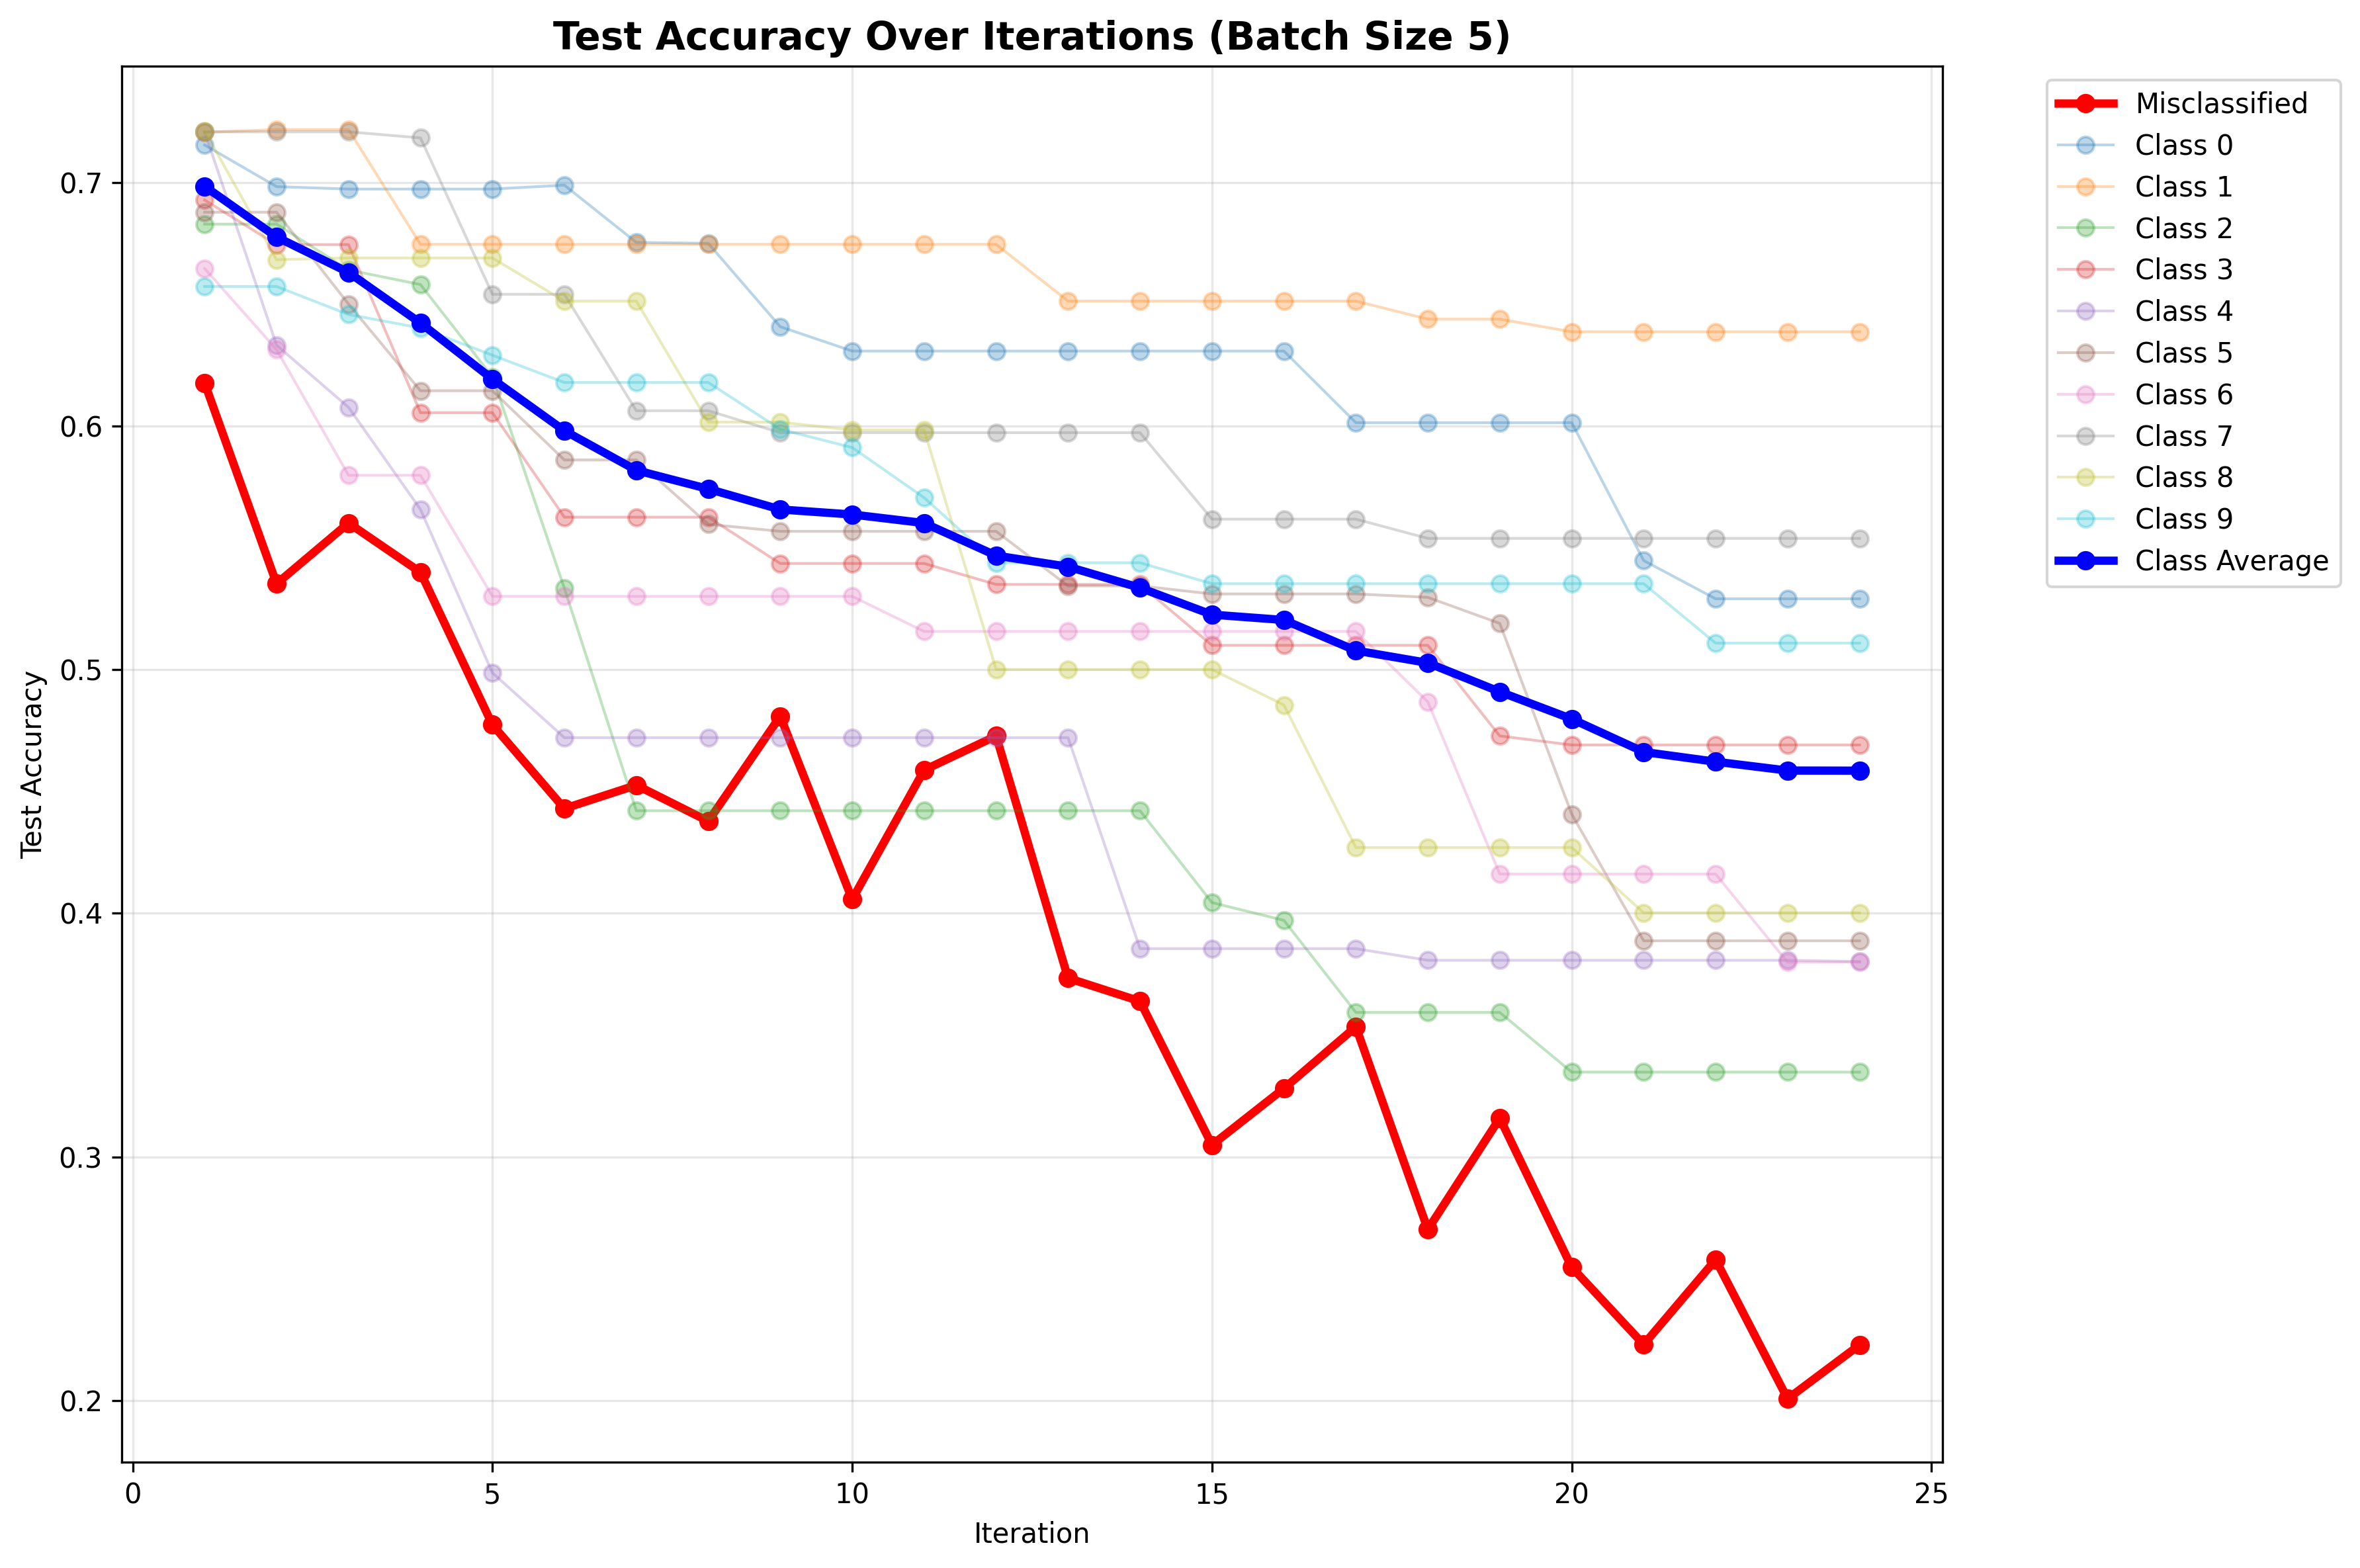
\includegraphics[width=\textwidth]{results/stochastic_analysis/batch_iterations/test_accuracy_batch_5.png}
	\caption{Test accuracy evolution for batch size 5 showing that early stopping around iteration 5 would preserve much higher global accuracy while maintaining excellent repair set performance.}
	\label{fig:early_stopping_batch_5}
\end{figure}

\begin{figure}[h]
	\centering
	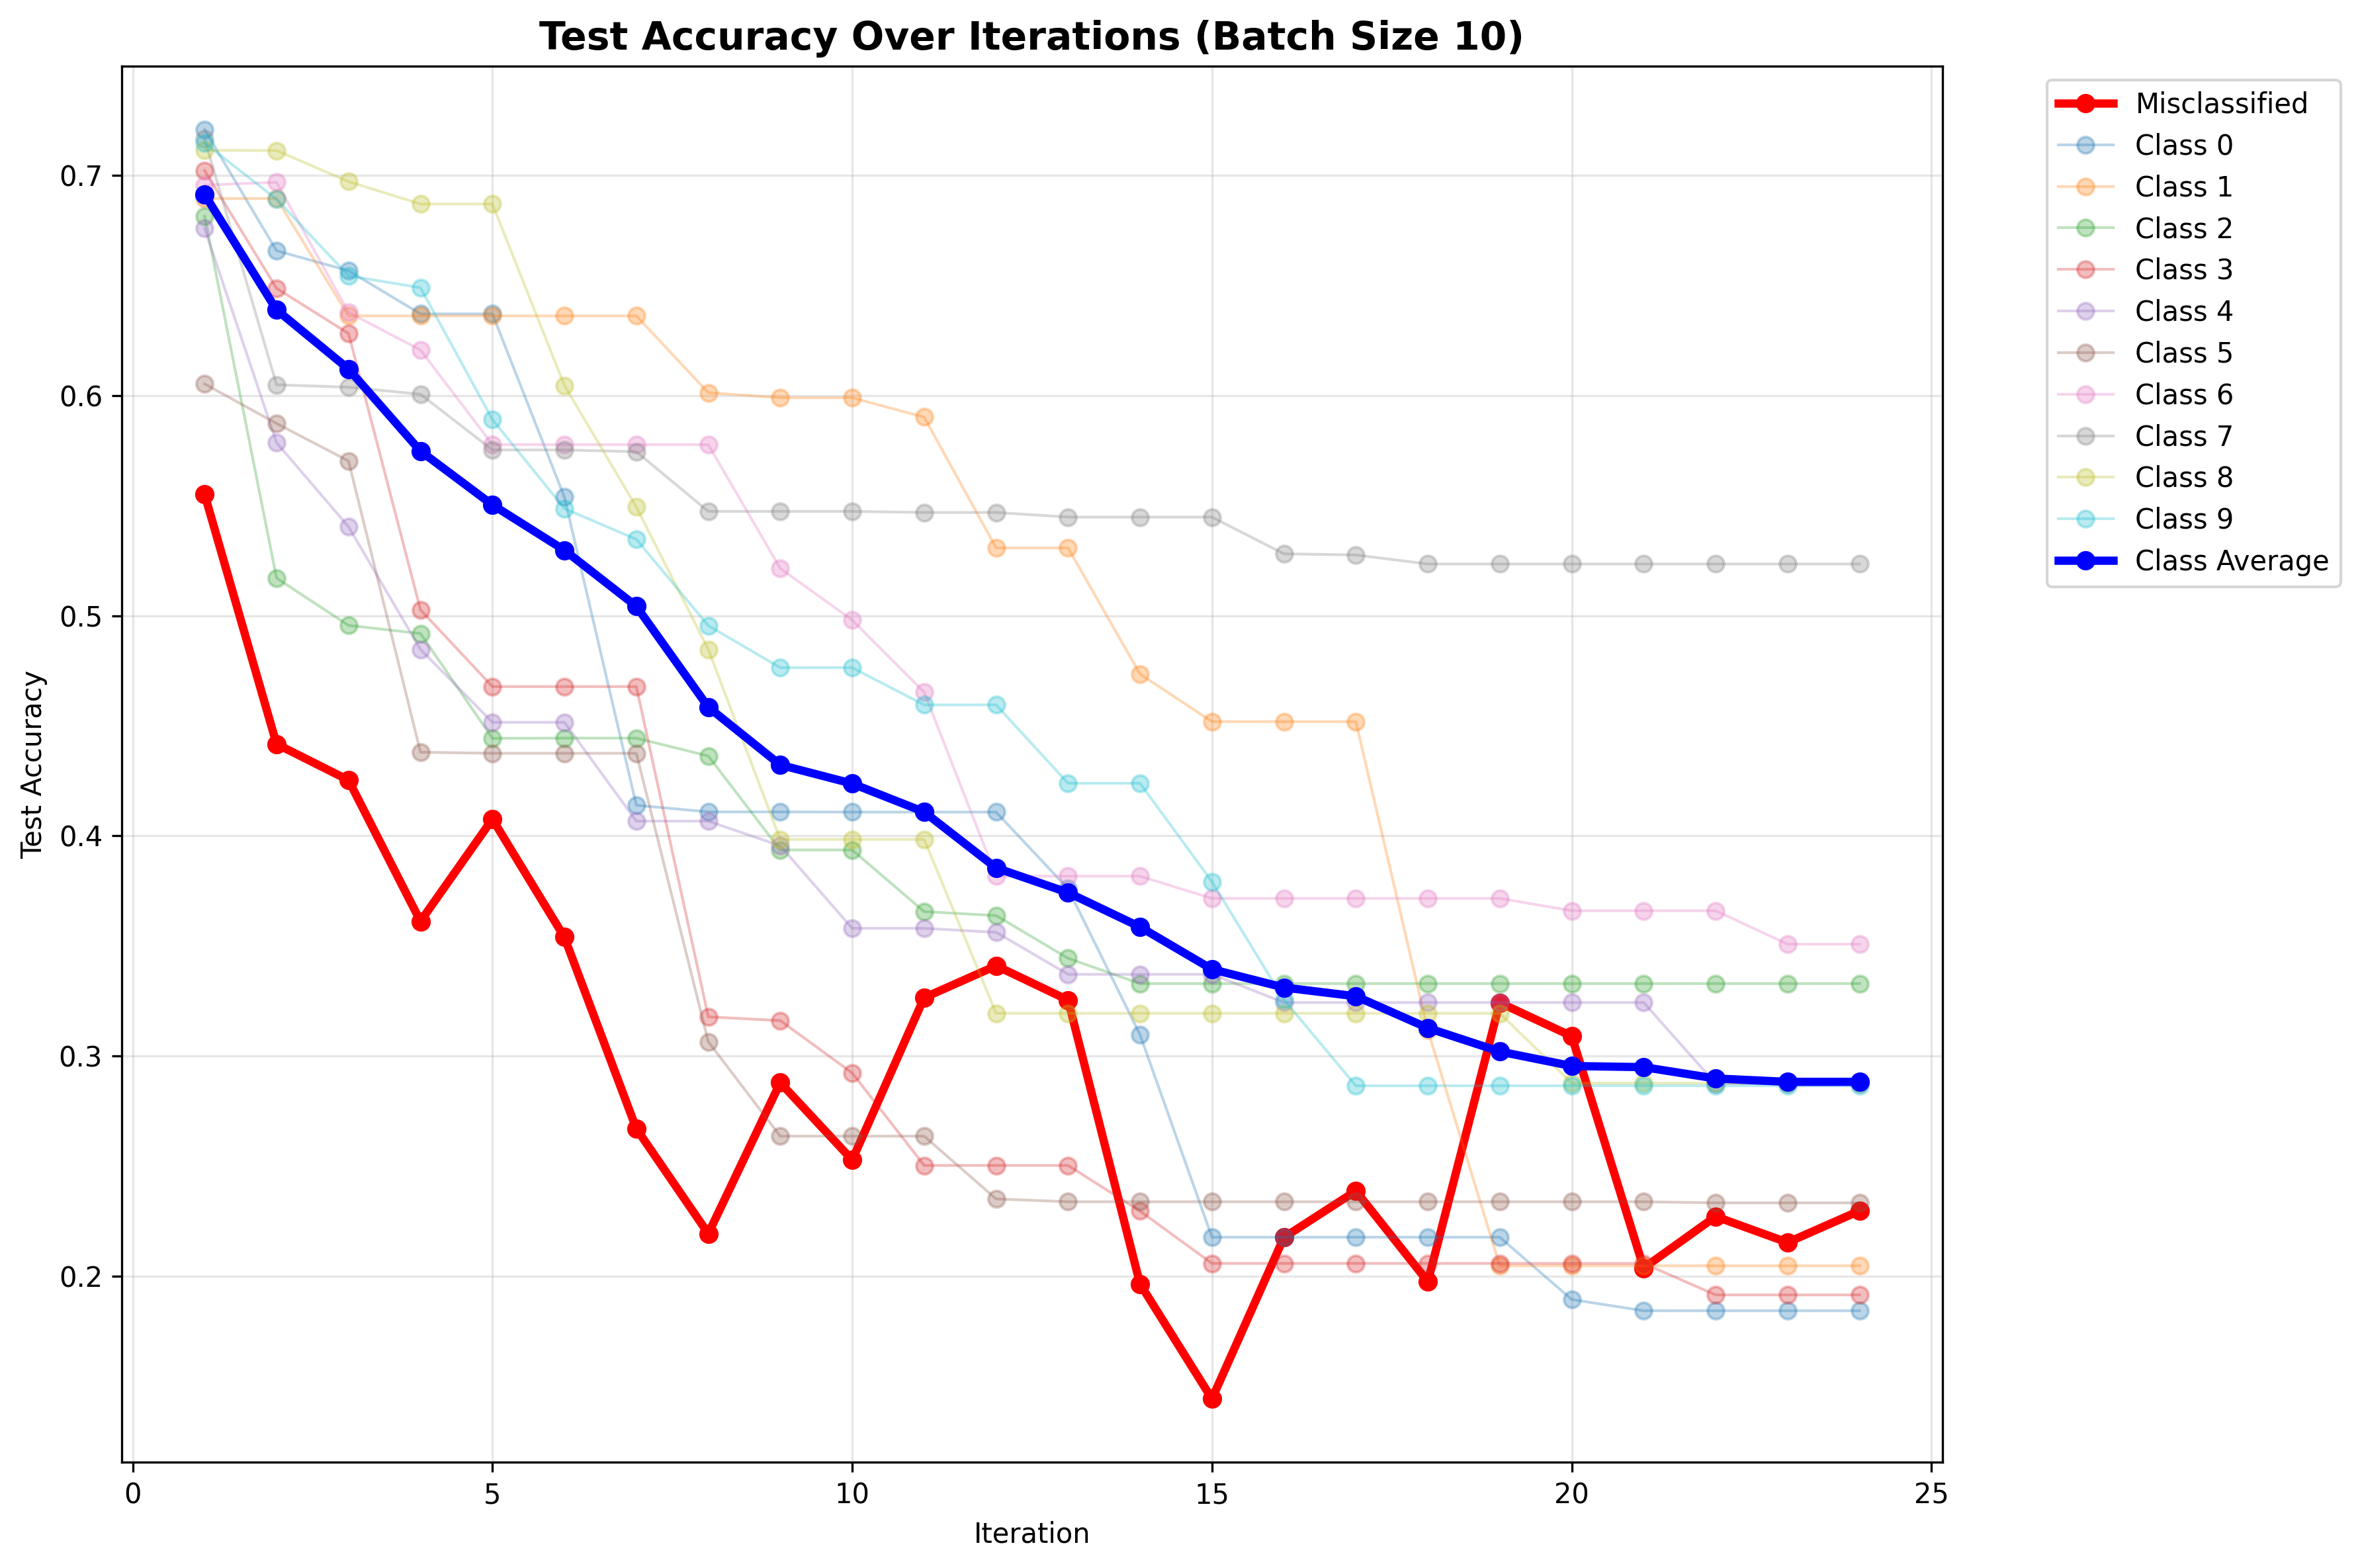
\includegraphics[width=\textwidth]{results/stochastic_analysis/batch_iterations/test_accuracy_batch_10.png}
	\caption{Test accuracy evolution for batch size 10 demonstrating similar early stopping opportunities to reduce drawdown.}
	\label{fig:early_stopping_batch_10}
\end{figure}

Key findings from our analysis show that:
\begin{itemize}
	\item \textbf{Rapid Convergence:} Class-homogeneous repairs reach 99\% repair set accuracy within 5 iterations
	\item \textbf{Early Stopping Benefit:} Stopping at iteration 5 preserves 60-65\% test accuracy vs. 45-29\% when running to completion
	\item \textbf{Batch Size Efficiency:} Both batch sizes 5 and 10 show similar convergence patterns, with batch 5 being slightly more stable
\end{itemize}

\subsection{Comparative Analysis and Implications}

Our experimental results reveal four key insights for neural network repair:

\begin{enumerate}
	\item \textbf{Size Limitations:} Repair set size is the primary limiting factor for repair feasibility. Success rates drop dramatically beyond 25 examples, while accuracy drawdown and computational cost scale unfavorably with size.

	\item \textbf{Homogeneity Advantage:} Class-homogeneous repair sets consistently outperform misclassified sets in both success rates and performance preservation, demonstrating the value of semantically coherent repair targets.

	\item \textbf{Stochastic Efficiency:} For class-homogeneous sets with small batch sizes (5-10), stochastic repair provides an efficient path to near-perfect local accuracy with predictable convergence.

	\item \textbf{Early Stopping Potential:} The rapid convergence of stochastic repair (within 5 iterations) presents an opportunity to significantly reduce global accuracy drawdown through early stopping strategies.
\end{enumerate}

\subsubsection{Practical Implications}

These findings have important implications for practical DNN repair deployment:

\begin{itemize}
	\item \textbf{Repair Set Curation}: Careful selection and grouping of repair examples by semantic similarity can substantially improve repair outcomes.
	\item \textbf{Size Limitations}: There exist practical upper bounds on repair set size beyond which the cure becomes worse than the disease.
	\item \textbf{Strategy Selection}: One-shot repair is generally preferable to iterative approaches for maintaining global model performance.
	\item \textbf{Monitoring Requirements}: Any repair strategy requires careful post-repair validation to ensure acceptable global performance retention.
\end{itemize}

\section{Conclusions and Future Work}

Our comprehensive evaluation of neural network repair strategies on AlexNet reveals fundamental trade-offs that must be carefully considered in practical applications. While both one-shot and stochastic repair approaches can achieve perfect local corrections, they impose significant costs on global model performance that scale with repair set size and heterogeneity.

The superior performance of class-homogeneous repair sets suggests that semantic coherence in repair examples is crucial for preserving model generalization. This finding points toward the importance of intelligent repair set curation and the potential value of clustering or grouping repair examples before applying corrections.

Our stochastic repair experiments demonstrate that iterative approaches, while intuitively appealing for their incremental nature, can actually be more destructive than one-shot repairs when applied naively. This counter-intuitive result highlights the complex dynamics of neural network parameter spaces and the difficulty of making localized corrections without global consequences.

Future work should focus on developing repair strategies that explicitly account for these trade-offs, potentially through:
\begin{itemize}
	\item Regularization techniques that preserve global decision boundaries while enabling local corrections
	\item Sophisticated layer selection heuristics that minimize repair impact on unrelated model functionality
	\item Adaptive repair strategies that adjust their approach based on repair set characteristics
	\item Multi-objective optimization frameworks that balance local repair success against global performance preservation
\end{itemize}

Ultimately, our results underscore the fundamental challenge of post-hoc neural network repair: achieving perfect local corrections while preserving global model capability remains an open and significant research problem.



% Add bibliography at the end
\bibliographystyle{plainnat}
\bibliography{references}

\end{document}
